% !BIB TS-program = biber

% -*- coding: utf-8 -*-
\documentclass{scrbook}[headings=normal]% Entspricht den Typografieregeln eines Buches
\usepackage{wbh-thesis} % Laden der Vorlage
\usepackage{blindtext}
\usepackage{listings}
\usepackage[automark,headsepline]{scrlayer-scrpage}
\renewcommand{\lstlistingname}{Quelltext}% Listing -> Quelltext
\renewcommand{\lstlistlistingname}{Quellcodeverzeichnis}

\usepackage{booktabs}
\usepackage{caption}
\usepackage[withpage]{acronym}
\usepackage{tabularx} 
\usepackage{xltabular}
\usepackage{hyperref}

\setlength{\extrarowheight}{4pt}


\KOMAoptions{%
    headsepline=true,   % header line
    footsepline=false,          % footer line
    plainheadsepline=false, % activate header line for plain pages
    plainfootsepline=false} % activate footer line for plain pages

\usepackage{mathtools}

\usepackage[framemethod=tikz]{mdframed}
\counterwithout*{footnote}{chapter}

% Shorthands
\newcommand*\iffdef{\overset{\text{def}}{\iff}}
\DeclarePairedDelimiter\abs{\lvert}{\rvert}
\DeclarePairedDelimiter\norm{\lVert}{\rVert}

\definecolor{WBH}{RGB}{0, 94, 166}

% Theorem
\mdtheorem[
  linecolor=WBH,
  frametitlefont=\sffamily\bfseries\color{white},
  frametitlebackgroundcolor=WBH,
]{Def}{Defintion}


\definecolor{codegreen}{rgb}{0,0.6,0}
\definecolor{codegray}{rgb}{0.5,0.5,0.5}
\definecolor{codepurple}{rgb}{0.58,0,0.82}
\definecolor{backcolour}{rgb}{0.95,0.95,0.92}

\definecolor{listingDartDocCommentColor}{rgb}{0.0,0.5,0.0}
\definecolor{listingDartTodoColor}{rgb}{0.6,0.0,0.0}
\definecolor{listingDartKeywordColor}{rgb}{0.1,0.0,0.5}

\usepackage{tikz}
\def\checkmark{\tikz\fill[scale=0.4](0,.35) -- (.25,0) -- (1,.7) -- (.25,.15) -- cycle;} 

\lstloadlanguages{% Check Dokumentation for further languages ...
csh,
Java
}
\definecolor{maroon}{rgb}{0.5,0,0}
\definecolor{darkgreen}{rgb}{0,0.5,0}

\lstdefinestyle{Codestyle}{
    backgroundcolor=\color{backcolour},   
    commentstyle=\color{codegreen},
    keywordstyle=\color{magenta},
    numberstyle=\tiny\color{codegray},
    stringstyle=\color{codepurple},
    basicstyle=\ttfamily\footnotesize,
    breakatwhitespace=false,         
    breaklines=false,                 
    captionpos=b,                    
    keepspaces=false,     
    columns=fullflexible,            
    numbers=left,                    
    numbersep=5pt,                  
    showspaces=false,                
    showstringspaces=false,
    showtabs=false,                  
    tabsize=1
}



\lstdefinelanguage{XML}
{
  morestring=[b]",
  moredelim=[s][\bfseries\color{maroon}]{<}{\ },
  moredelim=[s][\bfseries\color{maroon}]{</}{>},
  moredelim=[l][\bfseries\color{maroon}]{/>},
  moredelim=[l][\bfseries\color{maroon}]{>},
  morecomment=[s]{<?}{?>},
  morecomment=[s]{<!--}{-->},
  commentstyle=\color{darkgreen},
  stringstyle=\color{blue},
  identifierstyle=\color{red}
}

\definecolor{dkgreen}{rgb}{0,0.6,0}
\definecolor{gray}{rgb}{0.5,0.5,0.5}
\definecolor{mauve}{rgb}{0.58,0,0.82}

\definecolor{codegreen}{rgb}{0,0.6,0}
\definecolor{codegray}{rgb}{0.5,0.5,0.5}
\definecolor{codepurple}{rgb}{0.58,0,0.82}
\definecolor{backcolour}{rgb}{0.95, 0.95, 0.96}

\lstdefinelanguage{Dart} {
	morekeywords={Widget,class, if,int?,num, String,var,library,get, set,String,int,num ,await, async,  @override, return, Scaffold, AppBar, AppBar, TextField, ElevatedButton, GestureDetector, Card, Column, Center, Text, TextStyle,  MaterialApp,  extends, BuildContext, Tab, TabBarView, Icon, TabBar, with, InputDecoration, double, Map, bool,  List} ,
 	 morecomment=[l]{//},
	keywordstyle=\color{bluekeywords},
	commentstyle=\color{dkgreen}, 
	stringstyle=\color{mauve},
	numberstyle=\tiny\color{gray},
  	breaklines={true},
}


\definecolor{bluekeywords}{rgb}{0,0,1}
\definecolor{greencomments}{rgb}{0,0.5,0}
\definecolor{redstrings}{rgb}{0.64,0.08,0.08}
\definecolor{xmlcomments}{rgb}{0.5,0.5,0.5}
\definecolor{types}{rgb}{0.17,0.57,0.68}

\lstdefinelanguage{csh} {
morekeywords={ abstract, event, new, struct, as, explicit, null, switch,base, extern, object, this,bool, false, operator, throw,break, finally, out, true,byte, fixed, override, try,case, float, params, typeof,catch, for, private, uint,char, foreach, protected, ulong,checked, goto, public, unchecked,class, if, readonly, unsafe,const, implicit, ref, ushort,continue, in, return, using,decimal, int, async, await,sbyte, virtual,default, interface, sealed, volatile,delegate, internal, short, void,do, is,sizeof, while,double, lock, stackalloc,else, long, static, enum, namespace, EventArgs,string, Dictionary},
commentstyle=\color{greencomments},
morekeywords={partial, var, value, get, set},
keywordstyle=\color{bluekeywords},
stringstyle=\color{redstrings},
}
\usepackage{ltxtable}

\usepackage{acronym}


\lstset{style=Codestyle}

\usepackage{microtype}
\pagestyle{scrheadings}

\setlength{\headheight}{18pt}
\setlength{\footheight}{18pt}

\clearscrheadfoot

\ihead{\leftmark}
\ohead{\pagemark} 
\renewcommand*{\chapterpagestyle}{scrheadings}

\hyphenation{
platt-form-spe-zi-fi-schen
Code-erzeugung
Ereignis-erkennung
}

\newcommand{\Csharp}{%
  {\settoheight{\dimen0}{C}C\kern-.05em \resizebox{!}{\dimen0}{\raisebox{\depth}{\# }}}}




  \begin{document}

  \begin{titlepage}
\begin{center}
\newcommand{\HRule}{\rule{.9\linewidth}{.6pt}} % New command to make the lines in the title page

\vspace*{.06\textheight}
{\scshape\LARGE Wilhelm Büchner Hochschule}\vspace{1.5cm} % University name
\textsc{\Large Masterthesis}\\[0.5cm] % Thesis type

\HRule \\[0.4cm] % Horizontal line


\Large\textbf{ Realisierung eines Source-to-Source Compilers zwischen Xamarin.Forms und Flutter zur automatisierten Transformation bestehender mobiler 
Anwendungen}\par


\HRule \\[1.5cm] % Horizontal line
 
\begin{minipage}[t]{0.4\textwidth}
\begin{flushleft} \large
\emph{Author:}\\
Julian Pasqué % Author name - remove the \href bracket to remove the link
\end{flushleft}
\end{minipage}
\begin{minipage}[t]{0.4\textwidth}
\begin{flushright} \large
\emph{Betreuer:} \\
Dr. Thomas Kalbe % Supervisor name - remove the \href bracket to remove the link  
\end{flushright}
\end{minipage}\\[3cm]
 
\vfill


\large Verteilte und mobile Anwendungen\\[0.8cm] % Research group name and department name
\large Fachbereich Informatik\\[0.8cm] % Research group name and department name
\large Matrikelnummer: 902953 \\[0.8cm] % Research group name and department name
 
\vfill

{\large \today}\\[6cm] % Date
 
\vfill
\end{center}
\end{titlepage}  % Setzt die Titelseite
  \frontmatter        % Eigenschaften für den Vorspann setzen
  \renewcommand*\chapterheadstartvskip{}% removes space before chapter titles 

  \include{Abstract}  % Setzt die Titelseite

  \tableofcontents    % Setzt das Inhaltsverzeichnis
  \listoffigures      % Setzt das Abbildungsverzeichnis
  
  \listoftables       % Setzt das Tabellenverzeichnis
  \include{Abkürzungsverzeichnis}

  \let\footnotemark\relax
  \lstlistoflistings

  \mainmatter         % Eigenschaften für den Hauptteil setzen
  \KOMAoptions{headings=big}% restores default space before chapter titles

  \renewcommand*{\chapterpagestyle}{plain}
  \chapter{Einleitung}
Die Entwicklung von verschiedenen mobilen Geräten mit unterschiedlichsten Hardwarekomponenten und Betriebssystemen hat einen stark fragmentierten Markt ergeben.\footcite[Vgl.][S. 3]{Joorabchi2016}  Diese Situation hat einen direkten Einfluss auf die Softwareentwicklung, da die dedizierte Programmierung für die einzelnen Plattformen ressourcenintensiv ist.  Durch Realisierung von Web- und hybriden Apps können Softwareprojekte von der darunterliegenden Plattform abstrahieren und plattformübergreifend verwendet werden.  Diese Anwendungen haben jedoch, wie schon ausführlich im wissenschaftlichen Diskurs ausgeführt,  eine schlechtere Performance und nur begrenzt Zugriff auf die plattformspezifischen Funktionalitäten.  \footcite[Vgl.][S. 110ff.]{Barton2016} 

Durch die Kombination der Vorteile von Web- und hybriden Anwendungen mit denen von nativen konnten Frameworks wie Xamarin.Forms und Flutter Programmierern die Möglichkeit bieten,  ihre Anwendungen auf mehreren Plattformen bereit zu stellen.  Diese Apps haben neben einer guten Performance auch Zugriff auf sämtliche plattformspezifischen Funktionalitäten.  Durch die Abstraktion von Hardware und Betriebssystem können Apps mit einer gemeinsamen Quelltextbasis und somit mit geringerem Ressourcenaufwand entwickelt werden. \footcite[Vgl.][S. 295]{Vollmer2017} 

Der Möglichkeit, Ressourcen zu sparen, steht das Risiko der Abhängigkeit gegenüber, da sich die oben genannten Frameworks zur Cross-Plattform-Entwicklung in den verwendeten Programmiersprachen sowie ihrer Arbeitsweise grundlegend unterscheiden.  Ein Wechsel zwischen den einzelnen Alternativen ist daher mit enormen Arbeitsaufwänden verbunden. \footcite[Vgl.][S. 64]{Wissel2017}  

\section{Motivation}
Im Mai 2020 hat Microsoft mit dem .NET \ac{maui} einen Nachfolger für das Xamarin.Forms Framework angekündigt, der im Herbst 2021 zusammen mit der sechsten Hauptversion des .NET Frameworks veröffentlicht werden soll. Zum aktuellen Zeitpunkt ist bereits bekannt, dass der Umstieg grundlegende Änderungen mit sich bringt und Anwendungen,  die mit Hilfe von Xamarin.Forms entwickelt wurden,  angepasst werden müssen.\footcite[Vgl.][Abgerufen am 28.10.2020]{Hunter2020}

Für Xamarin.Forms Entwickler wird es also unausweichlich sein,  tiefgreifende Modifizierungen an bereits realisierten Anwendungen vorzunehmen,  um in der Zukunft von Aktualisierungen zu profitieren.  Unternehmen und einzelne Programmierer stehen vor der Entscheidung,  ob ein Umstieg auf das leistungsfähige Flutter sinnvoller ist,  als die Anpassungen für das neue noch nicht erprobte .NET \ac{maui},  das federführend von einer Firma entwickelt wird,  welche leichtfertig mit der Abhängigkeit von Entwicklern umgeht.

Ein automatisierter Umstieg auf das von Google entwickelte Framework Flutter würde also nicht nur die Anpassungen an .NET \ac{maui} vermeiden,  sondern die mobile Anwendung auf eine vermeintlich zukunftssichere Basis stellen.  Denn obwohl Google in der Vergangenheit schon manche Projekte eingestellt hat,  wie zum Beispiel Google Nexus oder Google Hangouts,  ist damit bei Flutter aufgrund des Erfolges nicht zu rechnen.  Nach offizieller Aussage von Tim Sneath, dem Produkt Manager des Frameworks,  haben im Jahr 2020 mehr als zwei Milliotatanen Entwickler Flutter verwendet und über 50.000 mobile Anwendungen programmiert. \footcite[Vgl.][Abgerufen am 28.10.2020]{Sneath2020} Neben der hohen Verbreitung des Frameworks,  konnte das Portal Stackoverflow in seinen jährlichen Umfragen auch eine hohe Beliebtheit unter Softwareentwicklern in den Jahren 2019\footcite[Vgl.][Abgerufen am 28.10.2020]{Stack2019} und 2020\footcite[Vgl.][Abgerufen am 28.10.2020]{Stack2020} ermitteln.  Im März 2021 hat Google darüber hinaus die zweite Hauptversion von Flutter veröffentlicht,  welche zusätzlich Support für die Entwicklung von Webseiten zur Verfügung stellt. \footcite[Vgl.][Abgerufen am 28.10.2020]{GoogleFlutter2}


\section{Ziel der Arbeit}
Im Rahmen dieser Arbeit soll ein Source-To-Source Compiler zwischen den Frameworks Xamarin.Forms und Flutter realisiert werden, mit dessen Hilfe die folgende zentrale Forschungsfrage beantwortet werden soll: "Können Apps komplett automatisiert von Xamarin.Forms zu Flutter übersetzt werden, oder sind manuelle Arbeitsschritte erforderlich?"

\section{Gliederung}
Um diese Forschunsgfrage beantworten zu können, wird in Kapitel \ref{chap:Compiler} auf die theoretischen Grundlagen von Software-Übersetzern eingegangen.  Anschließend wird in Kapitel \ref{chap:CompilerEntwurf} auf den Entwurf des in dieser Arbeit zu implementierenden Compiler eingegangen, bevor in Kapitel \ref{chap:CrossPlattformFrameworks} die Unterschiede zwischen den Frameworks Xamarin.Forms und Flutter behandelt werden.  Die Unterschiede zwischen den Programmiersprachen werden in Kapitel \ref{chap:Programmiersprachen} behandelt. Darauf aufbauend wird in Kapitel \ref{chap:Realisierung} der Source-To-Source Compiler realisiert und in dem darauf folgen Kapitel \ref{chap:Qualitätssicherung} getestet bevor in Kapitel \ref{chap:FazitAusblick} die Forschungsfrage beantwortet und ein Fazit gezogen wird. 
  \chapter{Compiler}
\label{chap:Compiler}

Programmiersprachen dienen als Verständigungsmittel zwischen Programmierern und Rechenanlagen wie z.B Smartphones.  Diese Sprachen haben sich in der Vergangenheit dabei immer mehr an die  Terminologie eines bestimmtes Anwendungsgebietes angenähert. Durch diese Entwicklung eigneten sich Programmiersprachen direkt für die Dokumentation von entwickelten Algorithmen und Anwendungen, entfernten sich jedoch weiter von den Gegebenheiten des realen Rechners.\footcite[Vgl.][S. 15]{Schneider1975} Die Beziehung zwischen Softwareentwicklern und Rechenanlagen mit Hilfe von Programmiersprachen werden in Abbildung \ref{fig:Programmiersprachen als Schnittstelle} dargestellt. 

\begin{figure}[!ht]
 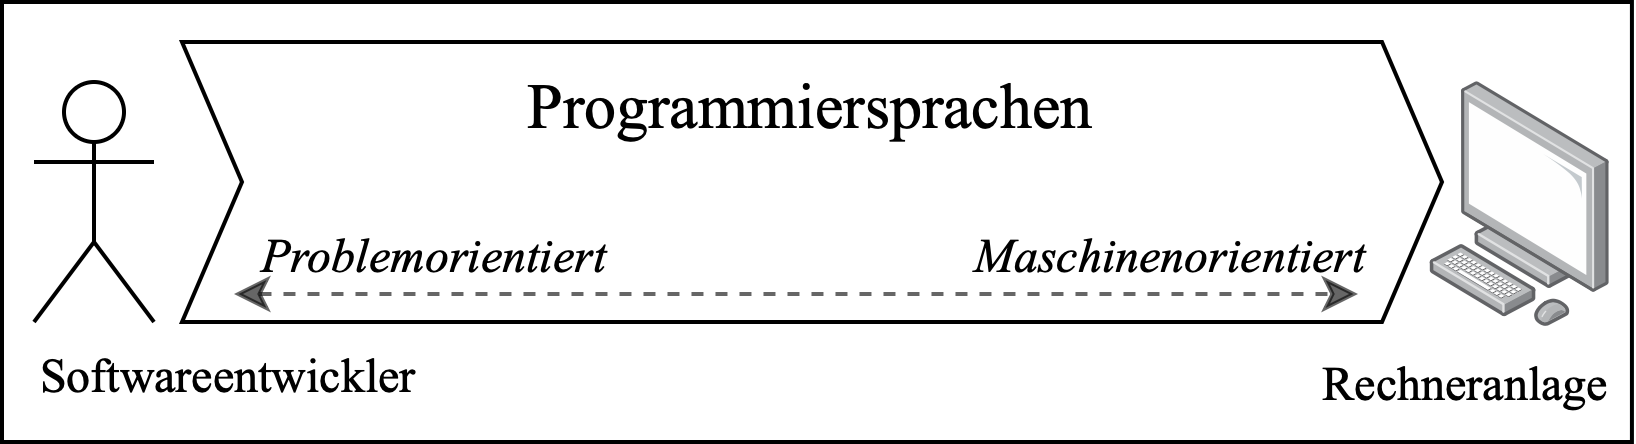
\includegraphics[width=\textwidth,height=\textheight,keepaspectratio]{Images/LanguageIntermediary.png}
 \caption{Programmiersprachen als Schnittstelle}
 \label{fig:Programmiersprachen als Schnittstelle}
\end{figure}

Für die Ausführung einer in einer problemorientierten Programmiersprache geschriebenen Anwendung ist es notwendig, die Sprache in eine maschinenorientierte Form zu überführen. \footcite[Vgl.][S. 15]{Schneider1975} Bereits im Jahre 1952 stelle Rutishauser fest,  dass Computer in der Lage sind,  diesen Übersetzungsvorgang selbst durchzuführen.\footcite[Vgl.][S. 312]{Rutishauser1952} 
Durch die Möglichkeit zur automatischen Übersetzung von problemorientierten Programmiersprachen konnten Hochsprachen entwickelt werden, die menschenfreundliche Sprachelemente anstatt Maschineninstruktionen verwenden. \footcite[Vgl.][S. 47]{Wagenknecht2014}
\section{ Grundbegriffe}
Diese historische Einführung zeigt,  dass Software zur automatisierten Übersetzung schon seit der Mitte des letzten Jahrhunderts thematisiert wurde, so hat sich in der Wissenschaft eine einheitliche Definition ergeben.  \citeauthor{Ullmann2008} beschreibt die sogenannten Compiler im Jahre \citeyear{Ullmann2008} wie folgt:\footcite[Vgl.][S. 1]{Ullmann2008} 
\begin{Def}[Compiler]
Ein Compiler ist ein Programm, welches ein anderes Programm aus einer Quellsprache in ein gleichwertiges Programm einer Zielsprache übersetzen kann.
\end{Def} 
\vspace{-1em}

Aus dieser Definition lässt sich ein für diese Arbeit relevanter Fakt ableiten: Compiler sind nicht ausschließlich Übersetzer  zwischen problemorientierten und maschinenorientierten Programmiersprachen.  Sie sind ausschließlich für die Übersetzung von einer Quellsprache in eine Zielsprache verantwortlich.  Auch wenn der Begriff Programm für jedermann geläufig ist,  kann es  passieren,  dass von verschiedenen Repräsentationen gesprochen wird.  So können alle drei der folgenden Begriffe als Programm bezeichnet werden: Der Quelltext,  das ausführbare Programm und der laufende Prozess auf einem Computer.  Für das weitere Verständnis dieser Arbeit ist mit dem Begriff Programm die ausführbare Anwendung auf den Smartphones des Anwenders gemeint.  

Neben der Übersetzung von problem- zu maschinenorientierter Sprache gibt es ebenfalls Compiler, die andere Ziele verfolgen. Dazu gehören zum Beispiel die sogenannten Binärübersetzer,  die den Binärcode eines Programmes für andere Rechner übersetzen, sodass er auf diesen ausgeführt werden kann.  \footcite[Vgl.][S. 27]{Ullmann2008} Ein
\ac{s2s} Compiler,  häufig auch als \glqq Transpiler\grqq{} bezeichnet,  ist ebenfalls eine besondere Ausprägung eines Compilers, die sich wie folgt definieren lässt.  \footcite[Vgl.][S. 1629]{IJCSIT2015}
\begin{Def}[Source-to-Source Compiler]
Ein Source-to-Source-Compiler ist ein Compiler, bei dem sowohl die Quellsprache als auch die Zielsprache eine Hochsprache ist.
\end{Def}
\vspace{-1em}

Der Begriff Hochsprache ist dabei ein Synonym für die bereits eingeführten problemnahen Sprachen wie zum Beispiel C++,  Java,  \Csharp  oder Dart und damit für den Menschen in einer lesbaren und änderbaren Form geschrieben sind. \footcite[Vgl.][S. 9]{Eisenecker2008} 

\section{Compiler Struktur}
Zur Übersetzung von Programmen bearbeiten Compiler zwei Teilaufgaben,  die Analyse und die Synthese. Während der Analyse wird das Programm in seine Bestandteile zerlegt und mit einer grammatikalischen Struktur versehen. Diese wird anschließend verwendet, um eine Zwischendarstellung zu generieren.  Dabei wird überprüft, ob das Programm syntaktisch und semantisch fehlerfrei ist oder ob der Programmierer Änderungen vornehmen muss. \footcite[Vgl.][S. 6f]{Ullmann2008} Der Begriff Syntax beschreibt den Aufbau eines Programmes,  sie legt fest wie Sprachelemente aus anderen Sprachelementen zusammengesetzt sind.  Im Gegensatz dazu beschreibt die Semantik die Bedeutung der Programmen und regelt die Bedeutung von Sprachelementen.  \footcite[Vgl.][S. 36]{Schneider1975}  Außerdem werden bei der Analyse Informationen über das Quellprogramm gesammelt und in der so genannten Symboltabelle abgelegt.  Die Synthese konstruiert aus der Zwischendarstellung und den Informationen aus der Symboltabelle das gewünschte Zielprogramm.  Der Teil des Compilers, der sich mit der Analyse befasst wird oft als Front-End bezeichnet, derjenige der für die Synthese zuständig ist als Back-End.  \footcite[Vgl.][S. 6f]{Ullmann2008}

Der Vorgang des Kompilierens lässt sich basierend auf diesen zwei Teilaufgaben nach \citeauthor{Ullmann2008} in mehrere Phasen unterteilen,  die in Abbildung \ref{fig:Compilerphasen} grafisch dargestellt sind und in diesem Abschnitt detailliert beschrieben werden.  \footcite[Vgl.][S. 6]{Ullmann2008}

\begin{figure}[!ht]
 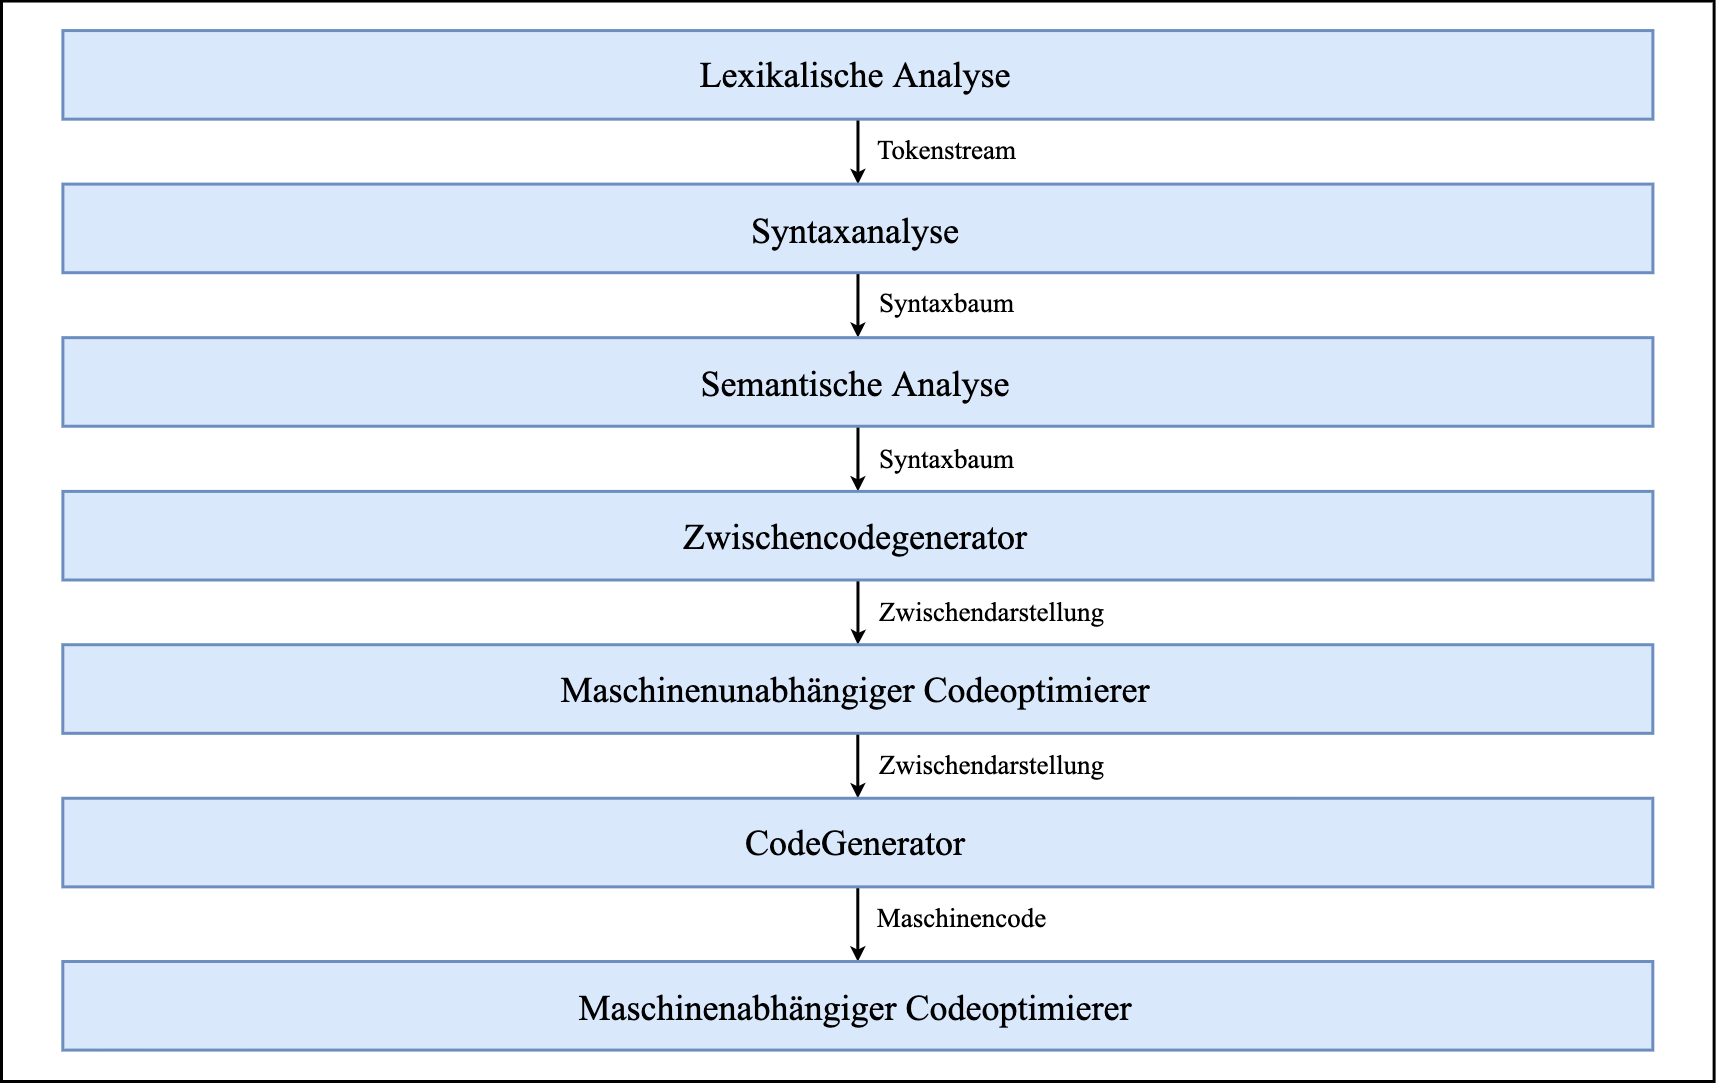
\includegraphics[width=\textwidth,keepaspectratio]{Images/Compiler/Phasen.png}
 \caption[Phasen eines Compilers]{Phasen eines Compilers\protect\footcite{Ullmann2008}}
 \label{fig:Compilerphasen}
\end{figure}
\footnotetext{Abbildung in Anlehnung an Ullman et al. 2008, S.6.}


\section{Lexikalische Analyse}
Die erste Phase eines Compilers ist die lexikalische Analyse,  die den Quelltext in Lexeme untergliedert.  Ein Lexem ist die Folge von Zeichen im Quellprogramm,  die als Instanz eines Tokens erkannt wurden.  Dabei ist ein Token ein Paar aus Namen und einem optionalen Attributwert,  wobei der Name zum Beispiel ein bestimmtes Schlüsselwort, oder eine Folge von Eingabezeichen sein kann und der Attributwert auf einen Eintrag in der Symboltabelle verweist.  \footcite[Vgl.][S. 135 f.]{Ullmann2008} In Tabelle \ref{tab:Tokens} werden einige beispielhafte Tokens aufgeführt sowie die Information darüber, aus welchen Lexemen diese extrahiert werden.

\begin{table}[!ht]
\begin{tabularx}{\textwidth}{l|X|l}
   \textbf{Token} & \textbf{Beschreibung} & \textbf{Lexem} \\
\hline
if             & Zeichen i,f           & if                      \\ 
comparison     & Vergleichsoperatoren  & \textless{}=            \\ 
id             & Buchstaben            & pi                      \\ 
number         & Numerische Konstanten    & 3.14159                  
\end{tabularx}
\caption[Token-Beispiele]{Token-Beispiele \protect\footcite{Ullmann2008}}
 \label{tab:Tokens}
\end{table}
\footnotetext{Vgl. Ullman et al.  2008, S. 137.}

Der Teil eines Compilers,  der die Lexikalische Analyse durchführt,  wird als Lexer bezeichnet.  Basierend auf der beschriebenen Arbeitsweise ist in \ref{fig:LexerResult} ein Beispiel dargestellt, das zeigt wie der Lexer aus einer Zeichenfolge mehrere Tokens mit den optionalen Attributwerten extrahiert.  
 
\begin{figure}[!ht]
 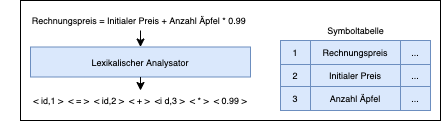
\includegraphics[width=\textwidth,keepaspectratio]{Images/Compiler/LexerResult.png}
 \caption[Lexer Beispiel]{Lexer Beispiel\protect\footcite{Ullmann2008}}
 \label{fig:LexerResult}
\end{figure}
\footnotetext{Abbildung in Anlehnung an Ullman et al. 2008, S.10.}

Der Lexer interagiert mit anderen Komponenten eines Compilers,  dies wird in Abbildung \ref{fig:LexerInteraktionen} visualisiert.  Klassischerweise wird der Lexer über den sogenannten Parser, welcher im nächsten Abschnitt eingeführt wird,  zur Übermittlung von Tokens aufgefordert,  dies wird in der Abbildung mit dem Aufruf "getNextToken" dargestellt.  \footcite[Vgl.][S. 135]{Ullmann2008} 

\begin{figure}[!ht]
 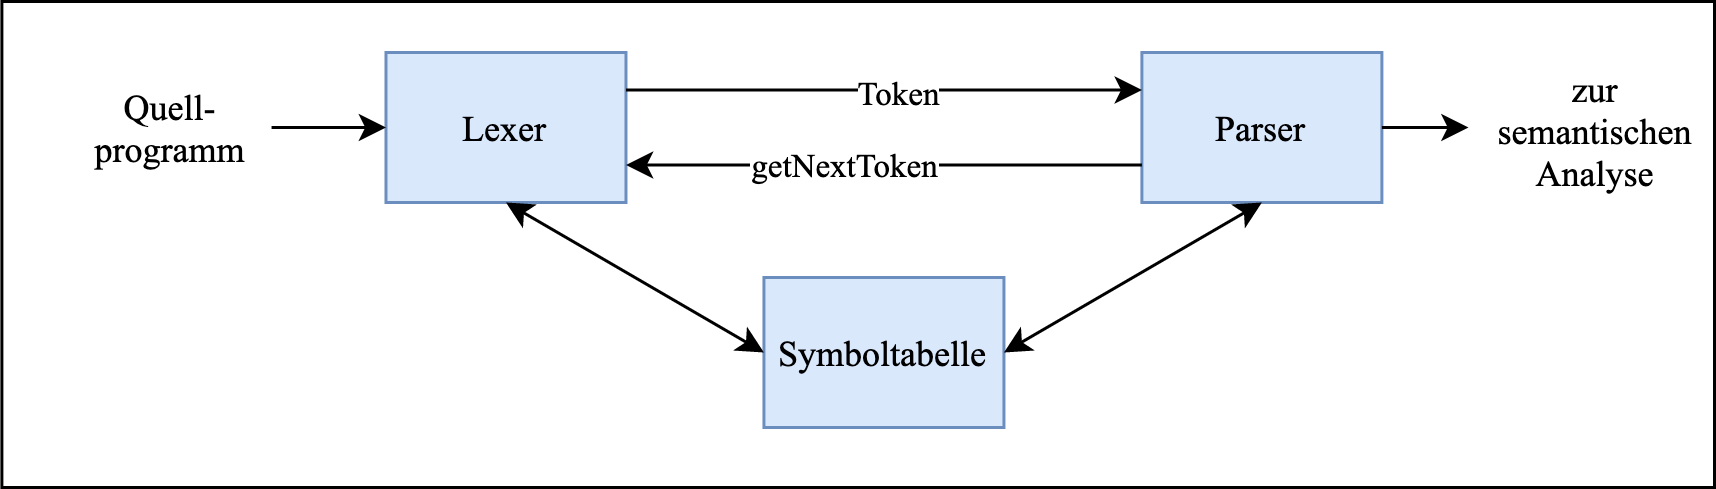
\includegraphics[width=\textwidth,keepaspectratio]{Images/Compiler/LexerParser.png}
 \caption[Interaktion zwischen Lexer und Parser]{Interaktion zwischen Lexer und Parser\protect\footcite{Ullmann2008}}
 \label{fig:LexerInteraktionen}
\end{figure}

Da der Lexer derjenige Teil des Compilers ist, der den Quelltext liest, kann er neben der Identifikation von Lexemen auch weitere Aufgaben übernehmen. So eignet er sich ideal zum Streichen von Kommentaren im Quelltext und zum Entfernen von Leerstellen,  wie Leerzeichen und Tabulatoren.  Zudem kann er gefundene Fehler den entsprechenden Zeilennummern zuordnen und dem Entwickler während der Kompilierung so einen genauen Hinweis auf den Ort des Fehlers geben. \footnotetext{Abbildung in Anlehnung an Ullman et al. 2008, S.135.} \footcite[Vgl.][S. 135.]{Ullmann2008} 
Häufig werden Lexer daher in zwei kaskadierende Prozesse unterteilt, einen für das Löschen von Kommentaren und Zusammenfassung von Leerraumzeichen und einen für die eigentliche lexikalische Analyse.  \footcite[Vgl.][S. 136.]{Ullmann2008} 

\section{Syntaxanalyse}
In der zweiten Phase, der Übersetzung, der Syntaxanalyse,  werden durch den bereits erwähnten Parser auch syntaktischer Analysator genannt,  die vom Lexer ausgegebenen Tokens in eine baumartige Zwischendarstellung überführt, die die grammatikalische Struktur der Tokens zeigt.  Diese Darstellung wird basierend auf ihrem Aussehen häufig als Syntaxbaum bezeichnet.  Die Knoten im Syntaxbaum stehen für eine Operation und die Kindknoten für die Argumente dieser Operation.  Die Anordnung der Operationen stimmt mit üblichen arithmentischen Konventionen überein,  wie zum Beispiel dem Vorrang der Multiplikation vor Addition. \footcite[Vgl.][S. 9]{Ullmann2008} Abbildung \ref{fig:ParserResult} zeigt die Erstellung eines Syntaxbaumes aus den Tokens  der Abbildung \ref{fig:LexerResult}.  Anhand des Knotens <id, 1> ist jederzeit über die Symboltabelle bekannt,  dass das Ergebnis der Rechnung an den Speicherort des Bezeichners Rechnungspreis abgelegt werden muss. \footcite[Vgl.][S. 9.]{Ullmann2008} 

\begin{figure}[!ht]
 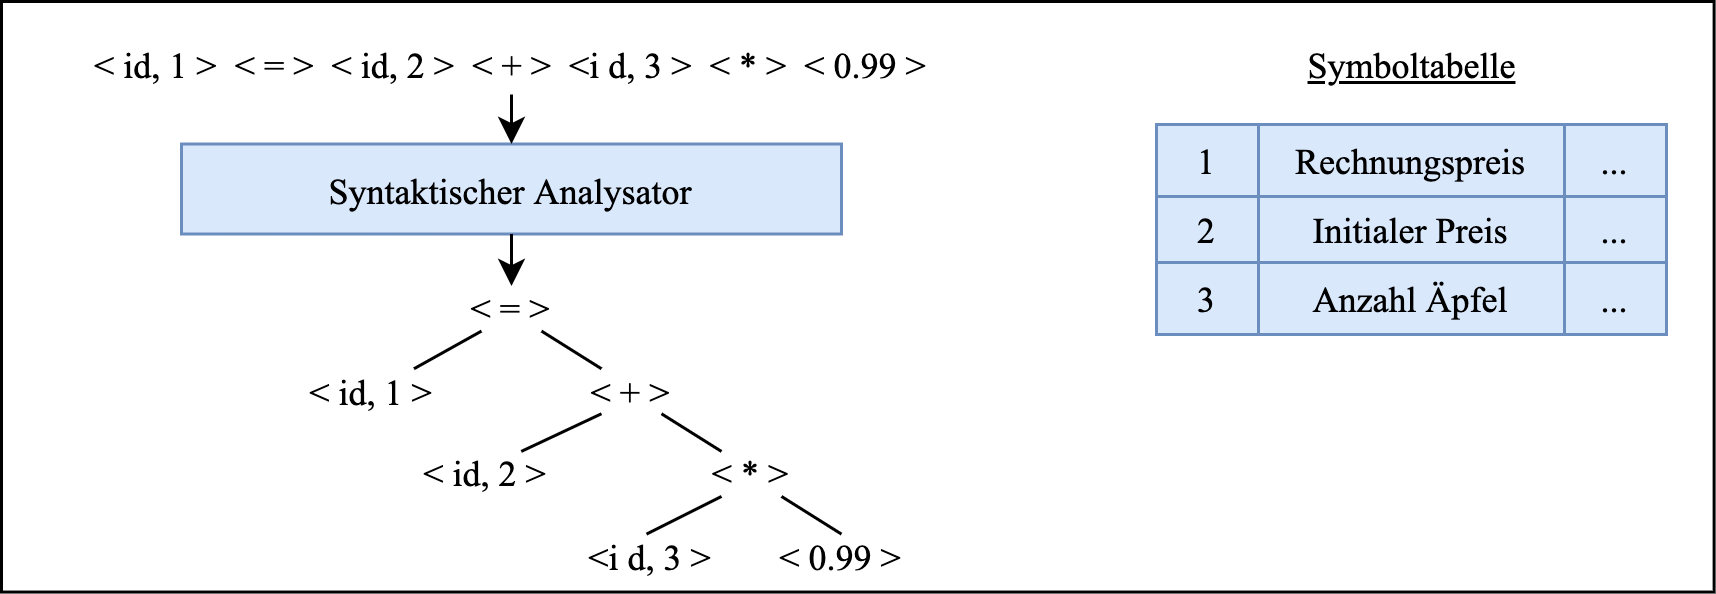
\includegraphics[width=\textwidth,keepaspectratio]{Images/Compiler/ParserResult.png}
 \caption[Syntaxbaum]{Syntaxbaum \protect\footcite{Ullmann2008} }
 \label{fig:ParserResult}
\end{figure}
\section{Semantische Analyse}

Bei der semantischen Analyse wird der Syntaxbaum  \footnotetext{Abbildung in Anlehnung an Ullman et al. 2008, S.10.}  als Aufgliederung der Programmkonstruktur,  zusammen mit den Informationen aus der Symboltabelle verwendet,  um das Quellprogramm auf semantische Konsistenz mit der Sprachdefinition zu überprüfen. \footcite[Vgl.][S. 157]{Wilhelm2012}.  Zudem werden hier Typinformationen gesammelt und zur späteren Verwendung im Syntaxbaum oder der Symboltabelle hinterlegt.  Auch findet eine Typüberprüfung statt die analysiert, ob jeder Operator die passenden Operanden hat.  So wird beispielsweise validiert,  ob ein Index eine Ganzzahl ist.  Es besteht die Möglichkeit, innerhalb des Baums Typkonvertierungen zu deponieren.  So wurde in dem bisherigen Beispiel die Anzahl Äpfel als Ganzzahl behandelt und wird für die Berechnung des Preises in Abbildung \ref{fig:Typ} zu einer Fließkommazahl konvertiert. \footcite[Vgl.][S. 9ff]{Ullmann2008}

\begin{figure}[!ht]
 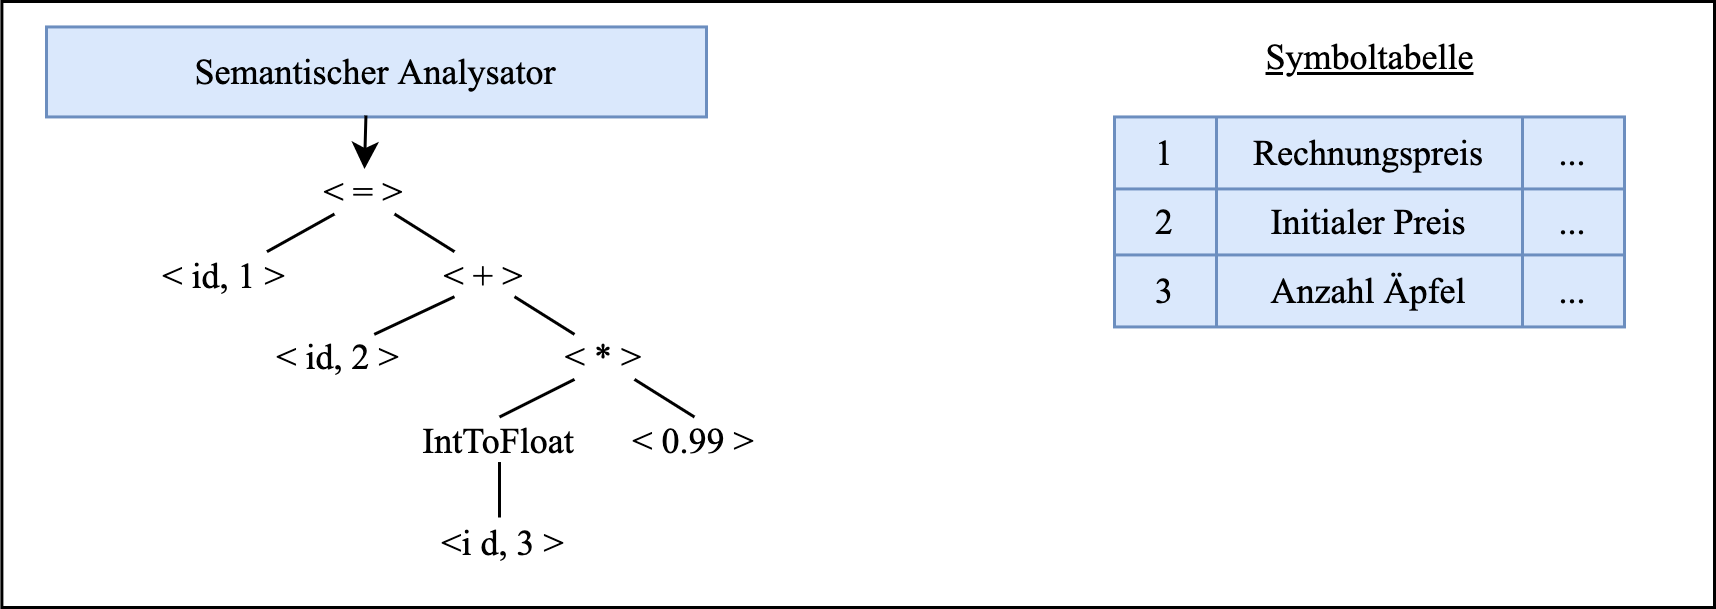
\includegraphics[width=\textwidth,keepaspectratio]{Images/Compiler/Type.png}
 \caption[Typüberprüfung]{Typüberprüfung \protect\footcite{Ullmann2008} }
 \label{fig:Typ}
\end{figure}
\footnotetext{Abbildung in Anlehnung an Ullman et al. 2008, S.10.} 
\section{Zwischencodeerzeugung}
Während der Übersetzung eines Programms  kann der Compiler mehrere Zwischendarstellungen in unterschiedlichsten Formen,  zum Beispiel wie die eines Syntaxbaums, erstellen.  
Nach der semantischen Analyse stellen viele Compiler eine maschinennahe Zwischendarstellung auf niedriger Abstraktionsebene her, die eigentlich für maschinenabhängige Aufgaben wie Befehlsauswahl geeignet ist. 
\begin{figure}[!ht]
 
\includegraphics[width=\textwidth,keepaspectratio]{Images/Compiler/Zwischendarstellungen.png}
 \caption[Zwischendarstellungen]{Zwischendarstellungen \protect\footcite{Ullmann2008} }
 \label{fig:Zwischendarstellung}
\end{figure}
\footnotetext{Abbildung in Anlehnung an Ullman et al. 2008, S.433.} 
Eine Zwischendarstellung, die von Compiler zu Compiler in Auswahl oder Entwurf unterschiedlich ist,  kann entweder eine tatsächliche Sprache sein,  oder aus internen Datenstrukturen bestehen, die von den Phasen des Compilers gemeinsam verwendet werden. Auch wenn C eine Programmiersprache ist, wird sie häufig als eine Zwischenform verwendet, da sie flexibel ist, zu effizientem Maschinencode kompiliert werden kann und ihre Compiler weitgehend verfügbar sind.\footcite[Vgl.][S. 433]{Ullmann2008}


\section{Codeoptimierung}
In dieser Phase wird der Code so optimiert, dass sich daraus ein besserer,  das heißt schnellerer oder ressourcenschonender Zielcode ergibt.  Der Umfang der Codeoptimierung schwankt dabei von Compiler zu Compiler erheblich.  \footcite[Vgl.][S. 11f]{Ullmann2008} 
Die Codeoptimierung, die ein Compiler vornimmt, ist im Laufe der Zeit wichtiger und  komplexer geworden. Grund für die zunehmende Komplexität sind die immer komplexeren Prozessorarchitekturen, die mehr Gelegenheiten bieten, die Ausführung des  Codes zu verbessern. Die gestiegene Bedeutung ergibt sich Beispielsweise aus der steigenden Anzahl an Kernen in modernen Computern und der Möglichkeit, Programme parallel auszuführen.\footcite[Vgl.][S. 20]{Ullmann2008}

\section{Codeerzeugung}
Die Überführung aus der Zwischendarstellung in die Zielsprache nennt man Codeerzeugung.  Hierbei muss die semantische Bedeutung des Quellprogramms erhalten und hochwertig dargestellt sein. Die größte Herausforderung ergibt sich aus der nicht komplett mathematischen Berechenbarkeit aller Prozesse bei der Überführung. Ein Beispiel wäre die Vergabe von Registern,  die nicht effizient berechenbar sind.  In der Praxis müssen heuristische Techniken ausreichen- die guten, aber nicht unbedingt optimalen Code liefern.  Die Codeoptimierungs- und  Codeerzeugungsphasen können mehrfach durchlaufen werden,  bevor das Zielprogramm finalisiert ist. \footcite[Vgl.][S. 618f]{Ullmann2008}

\section{Der .NET Compiler Roslyn}
Für die Arbeit mit der Programmiersprache \Csharp  steht mit Roslyn ein Compiler zur Verfügung, der sich aus modularen Bibliotheken zusammensetzt.  Durch die Referenzierung dieser Bibliotheken können Programme auf den Funktionsumfang von Roslyn zugreifen.  So ist es möglich, den Compiler zu verwenden, ohne das Ziel zu haben, die Programmiersprache \Csharp  in plattformnahen Code zu übersetzen.  Dabei stehen die Bibliotheken über den Packetmanager Nuget für die Einbindung in eigene Projekte zur Verfügung.  Um diese Funktionalität zu gewährleisten,  unterteilt Rosyln die Übersetzung in mehrere Phasen,  welche wiederum einige der in diesem Kapitel beschriebenen Phasen zusammenfassen. Die erste Phase ist die Erstellung des Syntaxbaums, die zweite Phase ist die semantische Analyse gefolgt von der letzten Phase der Ausgabe der so genannten Intermediate Language als Zielsprache. \footcite[Vgl.][S. 1017]{Albahari2020}




  \chapter{Compiler Spezifikation}
\label{chap:CompilerEntwurf}
Zur Entwicklung eines möglichst effektiven Compilers ist es notwendig, die genauen Anforderungen zu ermitteln,  um dann passende Softwaretechnische Lösungen zu erarbeiten. \footcite[Vgl.][S.6]{Balzert2011} Im speziellen Falle besteht die Anforderung darin, vom Quellframework Xamarin.Forms in das Zielframework Flutter zu übersetzen,  welche beide für die Entwicklung von plattformunabhängigen Smartphone-Apps verwendet werden können.  Für eine genaue Spezifikation des zu realisieren Source-To-Source Compilers ist es notwendig, einen Überblick über das Compiler-Umfeld zu erhalten.  Dieses wird in Abbildung \ref{fig:CompilerArchitecture} visualisiert. 

\begin{figure}[!ht]
 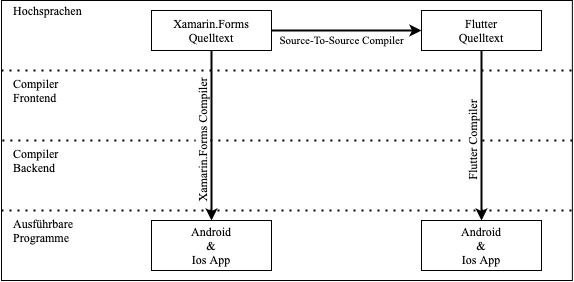
\includegraphics[width=\textwidth,keepaspectratio]{Images/CompilerArchitecture/CompilerStructure.png}
 \caption{Umfeld des Source-To-Source Compilerns}
 \label{fig:CompilerArchitecture}
\end{figure}

Wie auf der Abbildung erkennbar ist,  durchlaufen sowohl Xamarin.Forms als auch Flutter bei der Übersetzung zu mobilen Anwendungen die in Kapitel \ref{fig:S2SCompilerAufbau} erläuterten Phasen,  kurz dargestellt als Compiler Front- und Backend.  Der Source-To-Source Compiler ist in der Abbildung horizontal dargestellt,  was veranschaulichen soll,  dass sich sowohl die Quelle,  als auch das Ziel der Übersetzung auf einer Abstraktionsebene befinden.  Auch bei dieser Übersetzung sind die Compilerphasen aus dem vorherigen Kapitel anzuwenden.  So lässt sich die Abbildung \ref{fig:CompilerArchitecture},  wie in \ref{fig:S2SCompilerAufbau} dargestellt, um ein Front- und Backend erweitern.

\begin{figure}[!ht]
 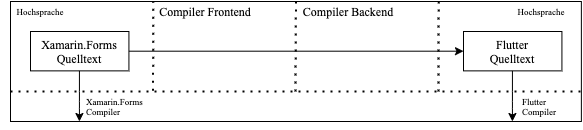
\includegraphics[width=\textwidth,keepaspectratio]{Images/CompilerArchitecture/S2SArchitecture.png}
 \caption{Source-To-Source Compiler Aufbau}
 \label{fig:S2SCompilerAufbau}
\end{figure}

Laut Definition von Compilern, erzeugen diese ein gleichwertiges Programm in einer Zielsprache.  Sowohl Xamarin.Forms als auch Flutter stellen mit Hilfe ihrer Compiler gleichwertige Programme in Form von mobilen Apps dar.  Da der Source-to-Source Compiler ebenfalls eine gleichwertige Darstellung erzeugt, ist anzunehmen, dass die übersetzte Ursprungs-App gleichwertig zu der übersetzten Flutter App ist. 

\section{Funktionseingrenzung}
Zur Beantwortung der Forschungsfrage ist es ausreichend, dass der Prototyp einen begrenzten Funktionsumfang hat.  Für eine zielführende Eingrenzung eignen sich die folgenden fünf Aspekte:

\begin{itemize}
\setlength\itemsep{-0.6em}
 \item Framework Version: Der in dieser Arbeit zu realisierende Prototyp soll ausschließlich das offiziell von Microsoft veröffentliche Xamarin.Forms in der Version 5.0.0.2012 zu Flutter übersetzten.  
 \item Erweiterungen von Dritten: Viele Firmen und einzelne Entwickler haben Erweiterungen für Xamarin.Forms programmiert.  Aufgrund der großen Anzahl und stetigen Veränderung dieser Erweiterungen, werden sie in dieser Arbeit nicht weiter betrachtet.  
 \item Plattformspezifischer Quelltext: Xamarin.Forms erlaubt die Verwendung von plattformspezifischem Quelltext,  der in dieser Arbeit keine Beachtung finden wird, da eine gleichwertige Darstellung in Flutter nicht garantiert werden kann. 
  \item Benutzerberflächen (UI): Für die Entwicklung von Benutzeroberflächen kann die Programmiersprache \Csharp verwendet werden,  jedoch hat die Alternative XAML (Extensible Application Markup Language) für Entwickler Vorteile, \footcite[Vgl.][Abgerufen am \today]{MicrosoftXAML2017} weswegen die Konstruktion von Benutzeroberflächen mit \Csharp in dieser Arbeit nicht berücksichtigt wird.  
  \item App-Styles: Für die visuelle Darstellung wird in dieser Arbeit ausschließlich das Design-System Material von Google unterstützt.  Da die Übersetzung von Darstellungsoptionen sehr aufwendig ist,  und für den in dieser Arbeit zu entwickelnden Prototypen nicht notwendig ist.  
\end{itemize}

Diese Eingrenzungen führen in Summe zu einer Vielzahl von nicht in Gänze übersetzbaren Xamarin.Forms Anwendungen.  Durch Erweiterungen des Compilers könnte diese Limitierung in Zukunft aufgehoben werden.  Im Rahmen dieser Arbeit wird eine mobile Xamarin.Forms Anwendung entworfen, die vollständig übersetzt werden kann, da sie keine der oben definierten Ausschlüsse verwendet. 


\section{Übersetzung von verschiedenen Dateien}
Durch seinen modularen Aufbau, kann der im letzten Kapitel eingeführte Roslyn Compiler die Phasen bis zur semantischen Analyse im zu entwickelnden Prototypen übernehmen.  Anschließend kann mithilfe des dabei typisierten Syntaxbaumes die Übersetzung in die Zielsprache durchgeführt werden.   Die Übersetzung mit Roslyn hat Grenzen,  die aus der Zusammensetzung von Xamarin.Forms Projekten resultiert.  Wie in Abbildung \ref{fig:CompilerStruktur} zu erkennen ist,  setzten sich Xamarin.Forms Projektmappen aus verschiedenen Dateien zusammen, von denen ausschließlich die Klassen beinhaltenden Dateien mit der Endung \glq cs\grq{}  analysiert werden können. 

\begin{figure}[!ht]
 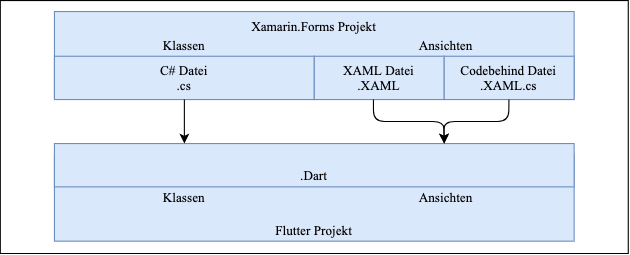
\includegraphics[width=14.5cm]{Images/Compiler/CompilerArchitecture.png}
 \caption{Compiler Struktur}
 \label{fig:CompilerStruktur}
\end{figure}

Neben den Klassen zeigt die Abbildung \ref{fig:CompilerStruktur},  dass auch Ansichten ein Teil von Xamarin.Forms Projekten sind.  Diese bestehen aus \glq XAML\grq{}  sowie \glq XAML.cs\grq{}  Dateien.  Alle Ausgangsdateien müssen zu Dart-Dateien kompiliert werden,  um ein Flutter Projekt als Ziel zu ergeben.  Die Zusammenführung von \glq XAML\grq{}  und \glq XAML.cs\grq{} Dateien ist dabei notwendig,  weil Flutter ohne sogenannte Codebehind Dateien auskommt. 

\section{Grafische Darstellung}
Damit Unternehmen und Entwickler ihre bestehenden Xamarin.Forms Anwendungen übersetzen können, muss eine Möglichkeit für die Interaktion mit dem Source-To-Source Compiler existieren.  Dieser Compiler ist zur einmaligen und nicht regelmäßigen Verwendung ausgelegt und braucht somit nicht in einer Entwicklungsumgebung integrieren werden.  Der Roslyn Compiler ist ausschließlich für das Betriebssystem Windows verfügbar,  die zu entwickelnde Oberfläche muss dementsprechend auf Windows Computern lauffähig sein.  Abbildung \ref{fig:UiMockup} zeigt einen Entwurf (engl. Mockup) der geplanten grafischen Benutzeroberfläche (GUI).

\begin{figure}[!ht]
 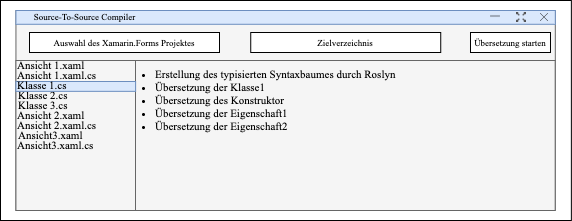
\includegraphics[width=\textwidth,keepaspectratio]{Images/CompilerArchitecture/Mockup.png}
 \caption{Mockup der grafischen Oberfläche}
 \label{fig:UiMockup}
\end{figure}

Im oberen Teil der GUI befindet sich eine Auswahl für das Quellprojekt und das Zielverzeichnis des Compilers.  Der untere Teil der Ansicht zeigt die Ausgabe des Übersetzers,  für die im linken Bereich alle bearbeiteten Dateien angezeigt werden.  Bei der Auswahl einer Datei werden in dem Bereich daneben alle vorgenommen Übersetzungsschritte aufgeführt.

\section{Quelltext Optimierung}
Die Optimierung des Quelltextes ist, wie in Kapitel \ref{chap:Compiler} beschrieben,  eine Phase der Kompilierung.  Im Gegensatz zu den dort beschriebenen Aspekten (Geschwindigkeit und Ressourcenschonung) sind für den Source-To-Source Compiler andere Faktoren wie der Austausch von Klassen und Methoden relevant,  da diese Ressourcenoptimierung später bei der Übersetzung durch den Flutter Compiler stattfinden.   
Der Bedarf zum Austausch von Klassen und Methoden resultiert aus unterschiedlichen Arbeitsweisen der Frameworks,  sodass eine einfache 1:1 Übersetzung nicht möglich ist.  Um dies zu visualisieren, wird folgend ein Quelltextbeispiel aus beiden Frameworks gezeigt,  die die selbe Funktionalität abbilden.

\lstinputlisting[label={lst:XFSelectImage},caption={Bilderauswahl in Xamarin.Forms}, language=csh]{SourceCode/Galery.cs}

\lstinputlisting[label={lst:FlutterSelectImage},caption={Bilderauswahl in Dart}, language=Dart]{SourceCode/Galery.Dart}

Beide Crossplatform Frameworks verwenden in diesem Beispiel unterschiedliche Klassen für die Auswahl eines Bildes aus der Smartphonegalerie.  Daher ist es notwendig,  beide Frameworks zu analysieren und die genauen Unterschiede zwischen den Arbeitsweisen zu verstehen.  Zu diesem Zweck werden im nachfolgenden Kapitel sowohl die Frameworks als auch deren Programmiersprachen analysiert.  Hieraus resultiert das Verständnis, inwiefern sich Benutzeroberflächen und Sprachen unterscheiden und wie diese übersetzt werden können.

Source-To-Source Compiler bilden eine Brücke zwischen zwei Hochsprachen.  Der für die Beantwortung der Forschungsfrage geplante Compiler soll darüber hinaus auch die Arbeitsweisen des Quellprogramms in das Zielprogramm übersetzen.  Das heißt, es soll versucht werden,  ein frameworkbasierte App in die Form eines Zielframeworks zu überführen. 




  
  \chapter{Technische Unterschiede zwischen Xamarin.Forms und Flutter}
\label{chap:CrossPlattformFrameworks}

Die Unterschiede zwischen den Frameworks werden im folgenden genauer betrachtet.  Für den technischen Vergleich dient Xamarin.Forms als Grundlage.  Die Namen von Abschnitten und Unterabschnitten orientieren sich deshalb an dessen Terminologie.  In den jeweiligen Gliederungspunkten wird anschließend genauer betrachtet,  wie sich spezielle Arbeitsweisen oder Darstellungsoptionen in Flutter abbilden lassen. 

\section{Projektaufbau}
Xamarin.Forms weist eine andere Projektstruktur auf als Flutter,  das nur mit einem Projekt arbeitet.  Wärend das Flutter Projekt alle notwendigen Inhalte für iOS und Android inkludiert, \footcite[Vgl.][S. 113]{Biessek2019} setzt sich die sogenannte Lösung bei Xamarin.Forms aus mehreren Projekten zusammen.  Es gibt für jede Plattform ein dediziertes Projekt, das den plattformspezifischen Code,  Konfigurationen und Icons beinhaltet, sowie ein Projekt für den plattformunabhängigen Quelltext.   \footcite[Vgl.][S. 25f.]{Petzold2016} Icons und Konfigurationen werden bei Flutter in einem gleichen oder ähnlichen Format und nur in einem weiteren Projekt hinterlegt und lassen sich folglich migrieren.  


\subsection{Metadaten}
Zu den Metadaten einer Anwendungen gehören unter anderem der Name der Anwendung,  Informationen wie die benötigte Betriebssystemversion, das \glq App Launcher Icon\grq, das auf dem Smartphonebildschirm angezeigt wird und die Berechtigungen,  die von der mobile Anwendung während der Ausführung beantragt werden können.  Diese Eigenschaften werden bei Xamarin.Forms innerhalb der nativen Projekte verwaltet.  In iOS können Änderungen mittels der Datei \glq Info.plist\grq{} definiert werden. \footcite[Vgl.][Abgerufen am \today]{MicrosoftInfoPlist2017} Android speichert Metadaten innerhalb der \glq AndroidManifest.xml\grq{}. \footcite[Vgl.][Abgerufen am \today]{MicrosoftManifest2018} Flutter verwendet für die Verwaltung der Metadaten die identischen Dateien,  daher ist es möglich,  diese aus dem Xamarin.Forms Projekt zu kopieren und innerhalb des Flutter Projektes zu sichern.  Dafür muss die \glq Info.plist\grq im Verzeichnis \glq ios/Runner/\grq{} und die \glq AndroidManifest.xml\grq{}  in \glq android/app/src/main/\grq{} gespeichert werden.  In diesen Dateien wird außerdem der Identifizierer der Anwendung definiert.  Durch eine Kopie der Konfigurationsdatei und Erhöhung der Versionsnummer wird eine spätere Kompilierung der Flutter-App demnach als eine Aktualisierung der Xamarin.Forms App erkannt.  \footcite[Vgl.][Abgerufen am \today]{Rana2020}


\subsection{Bilder und Startbildschirm}
Innerhalb von Apps können Bilder das Benutzererlebnis verbessern und helfen,  eine Aktion zu veranschaulichen oder komplexe Botschaften zu verdeutlichen.  \footcite[Vgl.][Abgerufen am \today]{GoogleMaterialImages2020} In iOS und Android werden sie in verschiedenen Auflösungen bereit gestellt.  Das Betriebssystem wählt während der Laufzeit die beste Ressource basierend auf den Eigenschaften des Smartphonedisplays aus.  Xamarin.Forms verwendet die \acfp{api} der nativen Plattformen zum Laden lokaler Bilder und unterstützt daher die plattformspezifischen Funktionalitäten.\footcite[Vgl.][Abgerufen am \today]{MicrosoftXamImages2020} Zur Verwendung nativer Bilddateien müssen die Bilder in Xamarin.Forms zu jedem Anwendungsprojekt hinzugefügt werden und vom gemeinsamen Xamarin.Forms-Code referenziert werden.  Flutter verwendet im Gegensatz zu Xamarin.Forms keine nativen \acp{api},  sondern ein einfaches dichte-basiertes Format,  ähnlich dem von iOS.  Für die Anzeige von Bildern arbeitet Flutter mit sogenannten logischen Pixeln.  Alle Bilderressourcen können sich in einem beliebigen Ordner innerhalb des Projektes befinden, da Flutter keine vordefinierte Ordnerstrukturen hat. \footcite[Vgl.][Abgerufen am \today]{GoogleFlutterImages2020} Der Startbildschirm (engl. Splashscreen) ist der Einstiegspunkt der mobilen App.  Er dient als Ladebildschrim und wird bei Xamarin.Forms in den plattformspezifischen Projekten gespeichert und kann ähnlich wie die \glq Info.plist\grq{}- und die \glq AndroidManifest.xml\grq{}-Dateien in das Flutter Projekt kopiert werden,  da die technische Implementierung identisch ist. \footcite[Vgl.][Abgerufen am \today]{GoogleSplash2020} 


\subsection{Benutzerdefinierte Schriftarten}
Eine Schriftart (engl. Font) wird verwendet,  um das Design und den Inhalt so klar und effizient wie möglich darzustellen,  dafür haben Android und iOS  eine Vielzahl vorinstalliert.  Wenn eine mobile App jedoch auf eine benutzerdefinierte Schriftart zurückgreifen möchte muss diese mit der Anwendung mitgeliefert werden.  In Xamarin.Forms mussten Fonts bis zum Jahre 2020 in jedem nativen Projekt referenziert werden.  Seit der Version 4.5 können diese Dateien auch plattformübergreifend verwendet werden und befinden sich daher innerhalb des geteilten Projekts. \footcite[Vgl.][Abgerufen am \today]{Versluis2020}  In Flutter werden die Fonts wie in der neueren Version von Xamarin.Forms in einem Ordner abgelegt. \footcite[Vgl.][Abgerufen am \today]{GoogleFlutterFonts2020}  Eine Verwendung des Schriftsatzes \glq MyCustomFont\grq{} in Flutter wird in Quelltext \ref{lst:FlutterFont} dargestellt.  

\lstinputlisting[label={lst:FlutterFont},caption={[Flutter Verwendung von Schriftsätzen]{Flutter Verwendung von Schriftsätzen\footcite[In Anlehnung an][Abgerufen am \today]{GoogleFlutterPackages2020}}}, language=Dart]{SourceCode/Fonts.Dart} 

\subsection{Plattformspezifischer Quelltext}
In\footcitetext[Quelltext in Anlehnung an][Abgerufen am \today]{GoogleFlutterFonts2020} den Ausschlusskriterien des dritten Kapitels wurde der plattformspezifische Quelltext von Xamarin.Forms für die Übersetzung exkludiert,  der Vollständigkeit halber sollen die Unterschiede zwischen den Plattformen jedoch trotzdem erwähnt werden.  Xamarin.Forms unterteilt nativen Quelltext in zwei Kategorien, den sogenannten \glq DependencyServices\grq{} die es erlauben,  Funktionenalitäten in den Plattformprojekten aus dem geteilten Code aufzurufen, \footcite[Vgl.][Abgerufen am \today]{MicrosoftDependencyService2017}  sowie \glq Custom Renderers\grq,  die es ermöglichen das Aussehen und Verhalten von Steuerlementen anzupassen. \footcite[Vgl.][Abgerufen am \today]{MicrosoftCustomRenderers2017} In Flutter wird für die Ausführung von plattformspezifischen Funktionalitäten auf \glq platform-channels\grq{} zurückgegriffen. \footcite[Vgl.][Abgerufen am \today]{GooglePlatformspecificCode2020} Für \glq Custom Renderer\grq{}  gibt es bei keine Alternative, da das Framework keine nativen Steuerelemente verwendet sondern Widgets anzeigt. 

\section{Erweiterungen}
Erweiterungen sind Programmergänzungen, die auch von externen Entwicklern beigetragen werden können.  Sie dienen der Reduzierung des Entwicklungsaufwandes, da nicht jede Funktionalität eigens implementiert werden muss.  Im .NET-Ökosystem können Xamarin.Forms-Projekte auf das Paketverwaltungssystem Nuget zugreifen,  um Erweiterungen zu einer App hinzuzufügen. \footcite[Vgl.][Abgerufen am \today]{MicrosoftXamNuget2020}  Bei Flutter wird für diesen Fall mit der pubspec.yaml Datei eine Referenz auf das ausgewählte Plugin gesetzt.  Dabei werden in Dart geschriebene Pakete von plattformunabhängigen Plugins unterschieden.  Diese Plugins können für Android (mit Kotlin oder Java) oder für iOS (mit Swift oder Objective-C) geschrieben sein. \footcite[Vgl.][Abgerufen am \today]{GoogleFlutterPackages2020} In Quelltext \ref{lst:Pubspecjaml} wird ein Auschnitt der pubspec.yaml Datei gezeigt, in welcher das in Unterabschnitt \ref{sec:nav} erwähnte Plugin \glq url\_launcher\grq{}   geladen wird.

%Kein Quelltext- ggf ändern.
\lstinputlisting[label={lst:Pubspecjaml},caption={[Erweiterungen in Flutter]{Erweiterungen in Flutter\footcite[In Anlehnung an][Abgerufen am \today]{GoogleFlutterPackages2020}}}, language=Dart]{SourceCode/Pubspec.yaml} 
\footcitetext[Quelltext in Anlehnung an][Abgerufen am \today]{GoogleFlutterPackages2020}In dem Beispiel muss das Plugin mindestens die Version 5.4 haben,  darf jedoch die Version 6 nicht überschreiten.  Aufgrund der Vielzahl an existierenden Erweiterungen für beide Frameworks ist es nicht möglich eine vollständige Gegenüberstellung zu erstellen.  Im Folgenden wird jedoch anhand von drei gängigen Anwendungsszenarien der Einsatz von Erweiterungen erläutert.

\subsection{Interaktion mit der Hardware}
Android und iOS nutzen einzigartige Betriebssystem- und Plattform-\acp{api},  auf die Xamarin.Forms Entwickler zugreifen können.  Mit der Erweiterung Xamarin.Essentials bietet Microsoft eine plattformübergreifende \ac{api}, auf die von gemeinsamem Code aus zugegriffen und die direkt auf der Plattform ausgeführt werden kann.  Der Dart Quelltext,  aus dem eine Flutter-App besteht, wird nicht auf der zugrundeliegenden Plattform, sondern nativ auf dem Gerät ausgeführt.  Es werden also nicht die iOS oder Android \acp{api}, benutzt.  Flutter Apps können über Plattformkanäle jedoch auch mit den nativen \acp{api} interagieren,  um beispielsweise Daten von Sensoren des Gerätes abzurufen.\footcite[Vgl.][Abgerufen am \today]{GooglePlatformspecificCode2020}

\subsection{Speicherung von Daten}
Ein wesentlicher Bestandteil jeder mobilen Anwendung ist die Fähigkeit,  Daten zu persistieren.  Manchmal handelt es sich dabei um große Datenmengen,  die eine Datenbank erfordern,  oft sind es aber auch kleinere Daten, wie Einstellungen und Präferenzen, die zwischen den Starts der Anwendung gespeichert werden müssen.  

Für die Speicherung in einer Datenbank können Xamarin.Forms Entwickler auf verschiedene Lösungsansätze zurückgreifen.  Zum einen \glq SQLite\grq{}, die am häufigsten verwendete Datenbank-Engine der Welt\footcite[Vgl.][Abgerufen am \today]{SQLiteConsortium2020},  oder \glq Realm\grq{},  eine Datenbank optimiert für mobile Endgeräte. \footcite[Vgl.][Abgerufen am \today]{MongoDBRealm2020} Beide Datenbanken stehen auch als Plugin für \glq Flutter\grq{} zur Verfügung, wobei SQLite ausgereift ist,\footcite[Vgl.][Abgerufen am \today]{Tekartik2020} während \glq Realm\grq{} erst am 5 November 2020 Support für Flutter angekündigt hat und noch nicht offiziell zur Verfügung steht. \footcite[Vgl.][Abgerufen am \today]{MongoDBFlutterSupport2020}

Die Xamarin.Essentials Erweiterung stellt Entwicklern das \glq Settingsplugin\grq{} bereit, welches die Sicherung von Präferenzen und App-Einstellungen erlaubt.  \footcite[Vgl.][Abgerufen am \today]{MicrosoftXamSettings2019} In Flutter wird für diese Speicherung mit Hilfe des Plugins \glq shared\_preferences\grq{}  auf die gleichen plattformspezifischen \ac{api} zugegriffen.  \footcite[Vgl.][Abgerufen am \today]{GoogleFlutterSharedPreferences2020}  Die Verwendung der gleichen \acp{api} ist ein wichtiger Faktor,  da die von Anwendern gespeicherten Daten,  auch nach einem Frameworkwechsel zu Flutter,  noch verfügbar sind. 

\subsection{Navigation zu anderen Anwendungen}
\label{sec:nav}

Mobile Anwendungen können die Möglichkeit zur Navigation zu anderen Apps realisieren.  Dafür greift Xamarin Forms auf ein bestimmtes \ac{uri}-Schema zurück, mit dem Ressourcen eindeutig bezeichnet werden.  Durch den Befehl \glq Launcher.OpenAsync("mailto://")\grq{}, der Bestandteil der Xamarin.Essentials Erweiterung ist,  wird z.B.  das Standardprogramm für E-Mails des Smartphones gestartet. \footcite[Vgl.][Abgerufen am \today]{MicrosoftLauncher2020}  Mithilfe des Plugins \glq url\_launcher\grq{} kann die Funktionalität zum Öffnen von anderen Anwendungen zu Flutter Apps hinzugefügt werden.\footcite[Vgl.][Abgerufen am \today]{Googleurllauncher2020} Die unterstützten \ac{uri}-Schemata und ihre Aktionen werden in Tabelle \ref{tab:URISChema} dargestellt.

\begin{table}[!ht]
\begin{tabularx}{\textwidth}{X|X}
   \textbf{\ac{uri}-Schemata} & \textbf{Aktion}  \\
\hline
	http:<URL>		       				&  	URL wird im Standardbrowser geöffnet 		\\ 
	mailto:<E-Mail Adresse>		       		&  	Erstellt eine Email an die angegebene E-Mail Adresse 		\\ 
	tel:<Telefonnummer>	       		&  	Ruft die Rufnummer an 		\\ 
	sms:<Telefonnummer>		       		&  	Schreibt eine SMS an die Rufnummer		\\ 
\end{tabularx}
\caption{Unterstützte Schemata des \glq url\_launcher\grq{} Plugins}
 \label{tab:URISChema}
\end{table}

\section{Lebenzyklus}
Durch das Navigieren zu anderen Anwendungen ändert sich der Status von Ausführung im Vordergrund zu Ausführung im Hintergrund.  Der aktuelle Status der App bestimmt die Handlungsoptionen.  Hat eine Vordergrund App die Aufmerksamkeit des Benutzers, ist sie priorisiert beim Zugriff auf die Systemressourcen, einschließlich der CPU.  Gleichzeitig muss eine Hintergrund-App möglichst inaktiv sein,  da sie sich außerhalb des Bildschirms befindet.  Mobile Anwendungen müssen auf Änderungen des Lebenszyklus-Status reagieren können, um ihr Verhalten entsprechend anzupassen.\footcite[Vgl.][Abgerufen am \today]{AppleLifecycycle2020} Xamarin.Forms bietet dafür die  drei Methoden \glq OnStart\grq{} , \glq OnResume\grq{} und \glq OnSleep\grq{} an,  die aufgerufen werden wenn sich der Status verändert. \footcite[Vgl.][Abgerufen am \today]{MicrosoftXamLifecycle2020} Bei Flutter kann auf die \glq didChangeAppLifecycleState\grq{} Methode zurückgegriffen werden, die bei Änderungsereignissen ausgelöst wird und die ebenfalls die drei Lebenszyklen beinhaltet. \footcite[Vgl.][Abgerufen am \today]{GoogleFlutterLifeCycle2020} 

\section{Ansichten}
Ansichten (engl. Views) sind visuelle Elemente, die in zwei Kategorien unterschieden werden können.  Steuerelemente (engl. Controls) sind für die Sammlung von Benutzereingaben oder die Ausgabe von Daten zuständig,  Layouts beinhalten eine Sammlung von Ansichten und sind für ihre visuelle Anordung auf der Benutzeroberfläche verantwortlich.  \footcite[Vgl.][Abgerufen am \today]{Ritscher2020} Im folgenden Abschnitt werden Xamarin.Forms und Flutter-Ansichten gegenübergestellt.  Damit soll ein Konzept für die Übersetzung von grafischen Benutzeroberflächen gelegt  und die Möglichkeiten des Austausches von Ansichten für den Compilers validiert werden.

\subsection{Layouts}
Ähnlich wie die Ansichten lassen sich auch die Layouts in zwei Kategorien unterteilen.  Den Ansichtsseiten (engl. Pages) sowie den generellen Layouts.  Die Pages nehmen den gesamten Bildschirm ein und werden in Abbildung \ref{fig:Xamarin.Forms Pages} dargestellt.\footcite[Vgl.][Abgerufen am \today]{MicrosoftXamPages2016}  

\begin{figure}[!ht]
 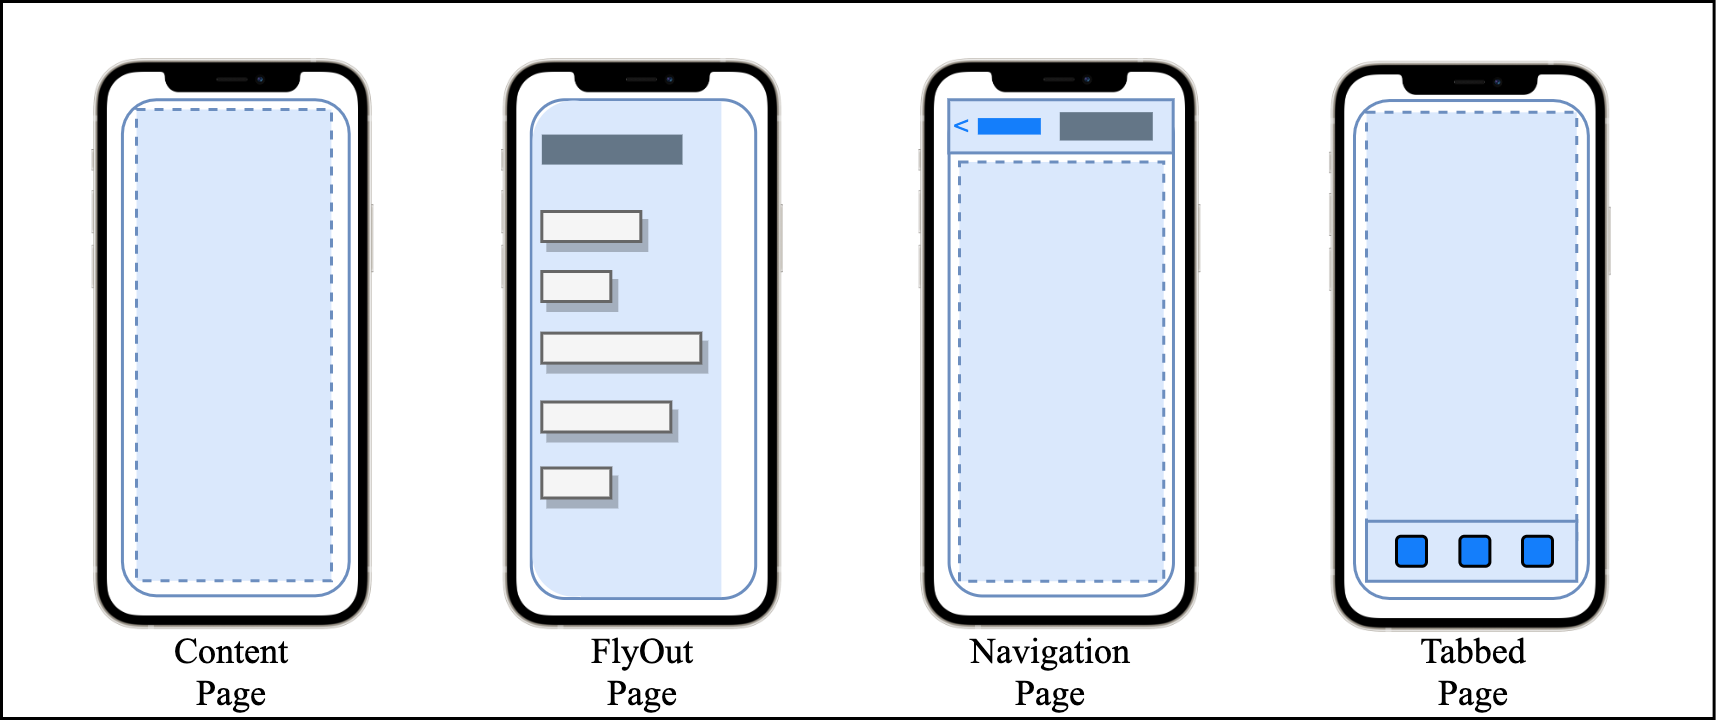
\includegraphics[width=\textwidth,height=\textheight,keepaspectratio]{Images/CrossPlattformFrameworks/XamarinFormsPages.png}
 \caption[Xamarin.Forms Pages]{Xamarin.Forms Pages\footcite{MicrosoftXamPages2016}}
 \label{fig:Xamarin.Forms Pages}
\end{figure}

Die \glq ContentPage\grq{} ist ausschließlich für die Anzeige einer weiteren Ansicht verantwortlich.  Die drei anderen Pages besitzen ein Navigationskonzept.  \footcitetext[Abbildung in Anlehnung an][Abgerufen am \today]{MicrosoftXamPages2016} Die \glq FlyOutPage\grq{} teilt den Bildschirm in zwei Bereiche, ein Bereich dient der Navigation.  Er enthält ein Menü das, wie im Namen enthalten, einfliegen kann.  Der zweite Bereich zeigt eine Detailansicht,  in welcher der Inhalt der angeforderten Seite geladen wird.  \glq NavigationPage\grq{} bietet eine Navigationsleiste, die einen Titel der aktuellen Seite und eine Navigationsschaltfläche beinhalten kann.  \glq TabbedPage\grq{} stellt die unterschiedlichen Seiten als Registerkarten dar. \footcite[Vgl.][Abgerufen am \today]{MicrosoftXamPages2016}
Die Ansichtsseiten befinden sich in der Regel innerhalb der \ac{xaml}-Datei auf der untersten Ebene, dem so genannten Wurzelknoten. Der Quelltext \ref{lst:TabbedPage} zeigt dies exemplarisch für eine \glq TabbedPage\grq{}.  

\lstinputlisting[label={lst:TabbedPage},caption={[Xamarin.Forms \glq TabbedPage\grq{} Definition]{Xamarin.Forms \glq TabbedPage\grq{} Definition\footcite[Quelltext in Anlehnung an][Abgerufen am \today]{MicrosoftXamTabbedView2020}}} , language=XML]{SourceCode/XamarinFormsTabbedPage.XAML}

\footcitetext[Quelltext in Anlehnung an][Abgerufen am \today]{MicrosoftXamTabbedView2020}Es wird eine \glq TabbedPage\grq{} mit zwei Registerkarten entworfen.  Eine Kombination mehrerer Navigationskonzepte ist  möglich,  das Beispiel zeigt eine Navigationsleiste innerhalb der Registerkarten. 

Die verfügbaren Eigenschaften der Ansichtsseiten unterscheiden sich je nach Einsatzszenario.  Im folgenden Quelltext \ref{lst:FlyOutPage} wird dies exemplarisch an der Realisierung einer \glq FlyoutPage\grq{} deutlich.  Anders als bei der \glq TabbedPage\grq{}, die aus einer Sammlung von Registerkarten besteht, finden sich im Quelltext die Eigenschaften \glq Flyout\grq{}  und \glq Detail\grq{}.

\lstinputlisting[label={lst:FlyOutPage}, caption={[Xamarin.Foerms \glq FlyoutPage\grq{} Definition]{Xamarin.Forms \glq FlyoutPage\grq{} Definition\footcite[Quelltext in Anlehnung an][Abgerufen am \today]{MicrosoftXamFlyOutPage2020}}} ,language=XML]{SourceCode/XamarinFormsFlyoutPage.XAML}

Im Gegensatz zu Xamarin.Forms kann Flutter auf der Wurzelebene nur den Style der App, \footcitetext[Quelltext in Anlehnung an][Abgerufen am \today]{MicrosoftXamFlyOutPage2020}
 nicht aber ein Navigationskonzept definieren.  Wie bereits in Kapitel \ref{chap:CompilerEntwurf} aufgeführt, wird in dieser Arbeit ausschließlich der Material Design Style unterstützt. \footcite[Vgl.][Abgerufen am \today]{FlutterForXFDevs} Quelltext \ref{lst:MaterialApp} zeigt die Realisierung einer MaterialDesign App in Flutter.

\lstinputlisting[label={lst:MaterialApp}, caption={[Flutter \glq MaterialApp\grq{} Definition]{Flutter \glq MaterialApp\grq{} Definition\footcite[Quelltext in Anlehnung an][Abgerufen am \today]{GoogleFlutterFirstApp2020}}}, language=Dart]{SourceCode/MaterialApp.Dart}

Der Vergleich zwischen den XML basierten \ac{xaml}-Dateien\footcitetext[Quelltext in Anlehnung an][Abgerufen am \today]{GoogleFlutterFirstApp2020} und den bei Flutter verwendeten Dart-Dateien verdeutlicht die Unterschiede in den verwendeten Sprachen zur Benutzeroberflächenentwicklung.  Die zentrale Idee hinter dem Flutter-Framework ist es,  eine Benutzeroberfläche aus Widgets aufzubauen.  Diese beschreiben das Aussehen der Anwendung basierend auf ihrem aktuellen Zustand.  Sobald sich der Status ändert, kann das Framework den neuen mit dem alten Status vergleichen, um grafische Veränderungen möglichst effektiv vorzunehmen. \footcite[Vgl.][Abgerufen am \today]{GoogleWidgets2020} Um in Flutter ein Navigationskonzept zu definiert ,  können verschiedene Widgets verwendet und verschachtelt werden,  wie in Quelltext \ref{lst:FlutterTabbedApp} beispielhaft für eine App mit Registerkarten visualisiert wird.

\lstinputlisting[label={lst:FlutterTabbedApp},caption={[Flutter \glq Tab Layout\grq{} Definition]{Flutter \glq Tab Layout\grq{} Definition\protect\footcite[Quelltext in Anlehnung an][Abgerufen am \today]{GoogleFlutterTabs2020}}}, language=Dart]{SourceCode/TabbedPage.Dart}
Die\footcitetext[Quelltext in Anlehnung an][Abgerufen am \today]{GoogleFlutterTabs2020}  deutlichen Unterschiede bei der Auswahl eines Navigationkonzeptes können überbrückt werden,  indem zu jeder Xamarin.Forms Page das entsprechende Flutter Widget gefunden wird.  Der Flutter-Widgetkatalog\footcite[Vgl.][Abgerufen am \today]{GoogleFlutterWidgetCatalog2020} und die Webseite "Flutter for Xamarin.Forms Developers"\footcite[Vgl.][Abgerufen am \today]{FlutterForXFDevs} wurde für die Recherche des Gegenstückes verwendet.  Entsprechende Ergebnisse der Suche können in Tabelle \ref{tab:ComparePAGESFlutter} abgelesen werden. 

\begin{table}[!ht]
\begin{tabularx}{\textwidth}{X|X}
   \textbf{Xamarin.Forms Page} & \textbf{Flutter Widget}  \\
\hline
	ContentPage            &           	\\ 
	FlyOutPage             & MasterDetailScaffold          	\\ 
	NavigationPage       & Scaffold         	 					\\ 
	TabbedPage            & TabBar und TabBarView 		\\ 
\end{tabularx}
\caption{Gegenüberstellung Pages}
 \label{tab:ComparePAGESFlutter}
\end{table}

Gegenüberstellungen in Tabellenform, von Xamarin.Forms Elementen und Flutter Widgets werden auch an anderer Stelle in diesem Kapitel zugunsten der Übersichtlichkeit verwendet.  Flutter Widgets, die im Text nicht expliziert aufgeführt werden,  sind den Xamarin.Forms Elementen in Funktionalität und Aussehen nahezu identisch.  Eine vollständige Referenztabelle,  die sich aus allen Einzelbetrachtungen zusammensetzt,  befindet sich in \hyperref[chap:Gegenueberstellung]{Anhang I} .

Die Navigation durch die Anwendung ist ein wichtiger Bestandteil und hängt wie beschrieben von der verwendeten Ansichtsseite ab.  Die \glq NavigationPage\grq{} bietet, eine hierarchische Navigation, bei der der Benutzer durch die Seiten vorwärts und rückwärts navigieren kann. \footcite[Vgl.][Abgerufen am \today]{MicrosoftXamNavigation2020} Flutter hat eine ähnliche Implementierung,  welche die Widgets  \glq  Navigator\grq{} und \glq  Routen\grq{} verwendet.  \footcite[Vgl.][Abgerufen am \today]{GoogleFlutterNavigation2020} 

Neben den Ansichtsseiten bietet Xamarin.Forms weitere Layouts,  die Steuerelemente zu visuellen Strukturen zusammenstellen.  Abbildung \ref{fig:Xamarin.Forms Layouts} präsentiert die gebräuchlichsten dieser Layouts. 

\begin{figure}[!ht]
 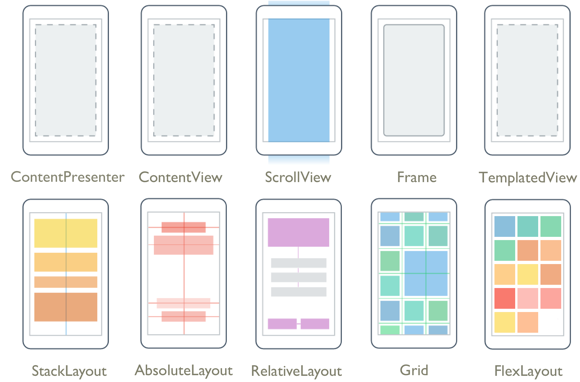
\includegraphics[width=\textwidth,height=\textheight,keepaspectratio]{Images/CrossPlattformFrameworks/XamarinFormsLayouts.png}
 \caption[Xamarin.Forms Layouts]{Xamarin.Forms Layouts\footcite{MicrosoftXamViews2020}}
 \label{fig:Xamarin.Forms Layouts}
\end{figure}

Die vorgestellten Layouts haben  unterschiedliche visuellen Eigenschaften und dienen als Sprachelemente von \ac{xaml} für den Entwurf von Benutzeroberflächen.  \footcitetext[Abbildung in Anlehnung an][Abgerufen am \today]{MicrosoftXamLayouts2018} \glq ContentView\grq{} enthält ein einzelnes untergeordnetes Ansichtselement und wird als Basisklasse für benutzerdefinierte Darstellungen verwendet.  Das Gestaltungselement \glq StackLayout\grq{} legt untergeordnete Elemente in einem entweder horizontal oder vertikal angeordneten Stapel ab.  Ein \glq Grid\grq{} positioniert seine untergeordneten Elemente in einem Raster aus Zeilen und Spalten,  es wird auch dafür verwendet,  Layouts und Steuerelemente übereinander zu legen.  Das \glq ScrollView\grq{} erlaubt das Verschieben von Bildschirminhalten und hat wie ein \glq ContentView\grq{} nur ein untergeordnetes Element.  
Neben diesen gängigen Layouts gibt es noch weniger verbreitete,  zum Beispiel  das \glq  Frame\grq{}, das einen Rahmen um ein visuelles Element zeichnet.  Das \glq AbsolutLayout\grq{},  platziert untergeordnete Elemente an bestimmten Positionen relativ zu ihrem übergeordneten Element.  Das \glq RelativeLayout\grq{} übernimmt die gleiche Aufgabe,  jedoch nur auf der Ebene des Layouts und untergeordneter Elemente. \footcite[Vgl.][Abgerufen am \today]{MicrosoftXamLayouts2018} Basierend auf diesen verfügbaren Layouts werden in Tabelle \ref{tab:XamLayouts} die entsprechenden Flutter Widgets entgegengesetzt.  

\begin{table}[!ht]
\begin{tabularx}{\textwidth}{X|X}
   \textbf{Xamarin.Forms Layout} & \textbf{Flutter Widget}  \\
\hline
	AbsolutLayout       		&  Positioned	 			\\ 
	ContentView       		&  StatelessWidget	 			\\ 
	Frame       					&  BoxDecoration     	 			\\ 
	Grid            				&  GridView oder Stack		\\ 
	ScrollView            		&  SingleChildScrollView		\\ 
	StackLayout       		&  Row und Column  	 			\\ 
	ReleativLayout           &  Positioned		\\ 
\end{tabularx}
\caption{Gegenüberstellung Layouts}
 \label{tab:XamLayouts}
\end{table}

Widgets haben zum Teil erweiterte oder abweichende Funktionalitäten, sodass Optimierungen durch den Compiler notwendig sind.  Damit das Layout \glq Grid\grq{} in Xamarin.Forms die Möglichkeit für einen Bildlauf bekommt, weil der Inhalt zu groß für die Darstellung auf einer Seite ist, wird das \glq Grid\grq{} in einem \glq ScrollView\grq{} verschachtelt. Dagegen bietet das \glq GridView\grq{} Widget von Flutter die Option des Scrollens automatisch an, wenn der Inhalt den sichtbaren Bereich überschreitet. \footcite[Vgl.][Abgerufen am \today]{GoogleFlutterGridView2020} Im Rahmen der Codeoptimierung muss das \glq ScrollView\grq{} in diesem Anwendungsfall entfernt werden.

\subsection{Steuerelemente}

Steuerelemente sind die sichtbaren Bausteine der Benutzeroberflächen,  beispielsweise Schaltflächen, Beschriftungen und Textfelder.  
Microsoft kategorisiert die Steuerelemente innerhalb der Frameworkdokumentation anhand ihrer primären Verwendung. \footcite[Vgl.][Abgerufen am \today]{MicrosoftXamViews2020} Diese Einteilung wird folgend übernommen,  obwohl eine klare Abgrenzung der  Steuerelemente zu Kategorien nicht uneingeschränkt möglich ist,  da einzelne zu mehreren Gruppierungen passen.


\subsubsection{Steuerelemente für die Präsentation}
Einige Steuerelemente sind ausschließlich für die Darstellung von Inhalten vorgesehen.  In Xamarin.\@Forms gibt es die folgenden  Darstellungssteuerelemente, für die eine Flutter Repräsentation notwendig ist.  Das Steuerelement \glq BoxView\grq{}zeigt in Xamarin.Forms ein einfarbiges Rechteck an.  Für die Darstellung von Texten wird auf \glq Label\grq{} zurückgegriffen.  Bilder können mit Hilfe des \glq Image\grq{}  Steuerelements angezeigt werden,  wobei diese aus verschiedenen Quellen, wie dem Web oder aus den Ressourcen der App geladen werden können.  Das Steuerelement \glq Map\grq{}  kann für die Anzeige von Karten innerhalb der mobilen Anwendung verwendet werden.  Um Web und HTML Inhalte innerhalb einer App visualisieren zu können, steht das \glq WebView\grq{}  Steuerelement bereit.  \footcite[Vgl.][Abgerufen am \today]{MicrosoftXamLayouts2018} Für die Steuerelemente kann nun eine Gegenüberstellung zwischen Xamarin.Forms Elementen und Flutter Widgets vorgenommen werden,  wie in Tabelle \ref{tab:ControlsVisualization} dargestellt.

\begin{table}[!ht]
\begin{tabularx}{\textwidth}{X|X}
   \textbf{Xamarin.Forms Steuerelement} & \textbf{Flutter Widget}  \\
\hline
	BoxView		       			&   	 SizedBox  		\\ 
	Image       						&	     Image	 			\\ 
	Label       						&  	Text 					\\ 
	Map            					&	   	Leamaps oder Google Maps \\ 
	WebView            			&  	webview\_flutter	\\ 
	Ellipse							&  	CustomPaint	\\ 
	Linie								&	  	CustomPaint	\\ 
	Path  							&  	CustomPaint	\\ 
	Polygon  						&  	CustomPaint	\\ 
	Polyline und Rectangle  &  	CustomPaint	\\ 
	Rectangle  					&  	CustomPaint	\\ 

\end{tabularx}
\caption{Gegenüberstellung Darstellungssteuerelemente}
 \label{tab:ControlsVisualization}
\end{table}
Zu zeichnende Elemente, wie die  \glq Ellipse\grq{}, \glq Linie\grq{}, \glq Path\grq{},  \glq Polygon\grq{},  \glq Polyline\grq{}  und \glq Rectangle\grq{} wurden nicht gesonders aufgeführt,  da diese bei Flutter auf die sogenannte Canvas der Benutzeroberfläche gezeichnet werden können.  \footcite[Vgl.][Abgerufen am \today]{GoogleFlutterCanvas2020} 

\subsubsection{Ereignisauslösende Steuerelemente}
Xamarin.Forms ist ein ereignisgesteuertes Framework. Die hier behandelten Steuerelemente stellen alle mindestens ein Ereignis zur Verfügung,  das durch die in Kapitel \ref{chap:CompilerEntwurf} erwähnten Codebehind Klassen abonniert werden kann.  Sobald ein  sogenanntes Event ausgelöst wird,  übermittelt das Framework diese Information an den Empfänger.   Die folgenden Steuerelemente werden bei Xamarin.Forms dieser Kategorie zugeordnet.  \glq Buttons\grq{} sind rechteckige Objekte,  die einen Text anzeigen und ein \glq clicked\grq{} Ereignis auslösen, nachdem sie von einem Anwender gedrückt wurden.  Mit \glq ImageButton\grq{} steht ebenfalls eine Variante zur Verfügung,  die ein Icon statt einem Text anzeigt.  Bei einem \glq RadioButton\grq{} wird eine Option aus einer Reihe von Möglichkeiten ausgewählt und löst ein Ereignis aus,  wenn sich die Benutzerauswahl ändert.  Ein weiteres Steuerelement ist \glq RefreshView\grq{}, das eine \glq PullToRefresh\grq{}  Funktionalität für Layouts mit Bildlauf anbietet.  Dabei wird durch das Herunterziehen des Seiteninhaltes der Wunsch zur Seitenaktualisierung  übermittelt.  Mithilfe der \glq Searchbar\grq{} haben Anwender die Möglichkeit, Inhalte  innerhalb der App zu suchen.  Nach der  Eingabe von Textzeichenfolgen kann per Schaltfläche,  oder Tastaturtaste, ein Ereignis ausgelöst und der eingegeben Text an die Codebehind-Datei weitergeleitet werden.  Tabelle \ref{tab:eventcommands} zeigt die ereignisauslösenden Steuerelementen von Xamarin.Forms und alternative Flutter Widgets.
\begin{table}[!ht]
\begin{tabularx}{\textwidth}{X|X}
   \textbf{Xamarin.Forms Steuerelemente} & \textbf{Flutter Widget}  \\
\hline
	Button		       				&  	ElevatedButton 		\\ 
	ImageButton		       		&  	IconButton 		\\ 
	RadioButton		       		&  	RadioButton 		\\ 
	RefreshView		       		&  	pull\_to\_refresh 		\\ 
	SearchBar		       			&  	flutter\_search\_bar 	\\ 
	SwipeView		       		&  	flutter\_slideable 		\\ 
\end{tabularx}
\caption{Gegenüberstellung ereignisauslösende Steuerelemente}
 \label{tab:eventcommands}
\end{table}

Flutter Widgets verhalten sich nicht exakt gleich wie die Steuerelemente von Xamarin.Forms.  Ein Beispiel ist die hier erwähnte SearchBar, die bei Flutter im Gegensatz zu Xamarin.Forms nicht frei platzierbar ist, sondern immer in der Navigationsleiste angezeigt wird. 

Die Beziehung zwischen Steuerelementen und Codebehind mittels Ereignissen wird  in den beiden folgenden Quelltextausschnitten demonstriert.  Der erste Ausschnitt zeigt  \ac{xaml} Quelltext,  durch welchen ein Button dargestellt werden kann.  Über die Eigenschaft clicked wird auf eine Methode in der XAML.cs Datei verwiesen,  die in dem zweiten Quelltextausschnitt abgebildet ist. 

\lstinputlisting[label={lst:XFVuttonDefinition},caption={Xamarin.Forms Button Initialisierung}, language=XML]{SourceCode/XamarinFormsButton.XAML}

\lstinputlisting[label={lst:XFEventHandler},caption={Xamarin.Forms Event Handler},  language=csh]{SourceCode/EventHandler.cs}

\subsubsection{Steuerelemente zur Textmanipulation}
In Xamarin.Forms stehen für die Arbeit mit Texten die Steuerelemente\glq Entry\grq{}zur  Eingabe von einzelnen und  \glq Editor\grq{} von mehreren Textzeilen bereit.  Tabelle \ref{tab:TextWidgets} zeigt die Gegenüberstellung zu Flutter Widgets.  

\begin{table}[!ht]
\begin{tabularx}{\textwidth}{X|X}
   \textbf{Xamarin.Forms Steuerelemente} & \textbf{Flutter Widget}  \\
\hline
	Entry		       		&  TextField	 		\\ 
	Editor		       	&  TextField	 		\\ 
\end{tabularx}
\caption{Gegenüberstellung textmanipulierender Steuerelemente}
 \label{tab:TextWidgets}
\end{table}
Wie in der Übersicht erkenntlich besitzt Flutter ausschließlich das Widget \glq TextField\grq{},  das beide Funktionalitäten der Xamarin.Forms Steuerelemente bündelt.  Standardmäßig bietet das \glq TextField\grq{} Widget die Eingabemöglichkeit für eine Zeile ähnlich dem \glq Entry\grq{} Steuerelement, kann aber durch das Setzen einer Eigenschaft erweitert werden.  Dies wird in Quelltext \ref{lst:FlutterTextField} dargestellt.

\lstinputlisting[label={lst:FlutterTextField},caption={Eingabefeld mit mehreren Zeilen in Flutter}, language=Dart]{SourceCode/FlutterTextField.Dart}

\subsubsection{Steuerelemente zur Wertsetzung}
Wersetzung bedeutet das Ergänzen von Steuerelmenten mit Eingaben durch den Anwender der App.  Die folgenden Steuerelemente bietet Xamarin.Forms in dieser Kategorie an.  Das \glq CheckBox\grq{}  Steuerelement ermöglicht dem Benutzer die Auswahl eines boole­schen Wertes (wahr, falsch).  Die gleiche Funktionalität, bei einem anderen visuellen Erscheinungsbild (siehe Abbildung  \ref{fig:SwitchCheckbox}) bietet der \glq Switch\grq{}.  

\begin{figure}[!ht]
 
\includegraphics[width=\textwidth,height=\textheight,keepaspectratio]{Images/CrossPlattformFrameworks/SwitchTextBox.png}
 \caption{Darstellung von den Steuerelementen \glq Checkbox\grq{} und \glq Switch\grq}
 \label{fig:SwitchCheckbox}
\end{figure}
Die beiden linken Darstellungen der jeweiligen Steuerelemente zeigen den Zustand mit dem boolschen Wert falsch,  die rechten wahr.

Ein  \glq Slider\grq{}  gewährt den Anwendern die Option einen Wert aus einem kontinuierlichen Bereich,  ein \glq Stepper\grq{}  aus einem Bereich von inkrementellen Werten auszuwählen.  Eine Datumsauswahl wird durch das \glq DatePicker\grq{} Steuerelement ermöglicht,  die Zeitauswahl mit \glq TimePicker\grq{}.  Die Tabelle \ref{tab:valuecontrols} präsentiert die gewohnte Gegenüberstellung von Xamarin.Forms Steuerlementen zu Flutter Widgets. 

\begin{table}[!ht]
\begin{tabularx}{\textwidth}{X|X}
   \textbf{Xamarin.Forms Steuerelemente} & \textbf{Flutter Widget}  \\
\hline
	CheckBox		       				&  Checkbox	 		\\ 
	Switch		       					&  Switch	 		\\ 
	Slider		       					&  Slider	 		\\ 
	Stepper		       				&  number\_inc\_dec	 		\\ 
	DatePicker		       			&  TextField mit Funktion		\\ 
	TimePicker		       			&  TextField mit Funktion	 		\\ 
\end{tabularx}
\caption{Gegenüberstellung wertsetzender Steuerelemente}
 \label{tab:valuecontrols}
\end{table}
 
Für die Steuerelemente \glq DatePicker\grq{}  und \glq TimePicker\grq{} steht kein entsprechendes Widget zur Verfügung.  Durch \glq TextField\grq{} und mithilfe einer Fingergeste wird eine Funktion aufgerufen, die den Auswahldialog für Datum und Uhrzeit öffnet und anschließend die Auswahl in das Textfeld einträgt.  Quelltext \ref{lst:FlutterTimePicker} repräsentiert diese Funktion in Dart am Beispiel einer Zeitauswahl. 
\newpage
\lstinputlisting[label={lst:FlutterTimePicker},caption={[Verwendung von Timepickern in Flutter]{Verwendung von Timepickern in Flutter\protect\footcite[Quelltext in Anlehnung an][Abgerufen am \today]{GoogleTimepicker2020}}}, language=Dart]{SourceCode/FlutterTimePicker.Dart}

Die \footcitetext[Quelltext in Anlehnung an][Abgerufen am \today]{GoogleTimepicker2020}
gesetzten Werte können bei Xamarin.Forms aus den Codebehind Klassen abgefragt werden,  um den Status eines Steuerelementes zu ermitteln.  Das Abrufen von Informationen in Flutter wird von speziellen Widgets,  beispielsweise dem \glq TextEditingController\grq{} durchgeführt.

\subsubsection{Aktivitätsandeutende Steuerelemente}

In mobilen Anwendungen kann es aufgrund der limitierten Hardware Ressourcen und begrenzten Netzwerkanbindung zu zeitaufwendigen Aktionen kommen.  Zur Visualisierung dieser Ladezeit stehen in Xamarin.Forms die folgenden Steuerelemente zur Verfügung.  Der \glq ActivityIndicator\grq{} zeigt durch eine Animation,  dass eine langwierige Aktivität ausführt wird,  die \glq ProgressBar\grq{} kann mittels Ladebalken auch den Fortschritt darstellen.  Die Tabelle \ref{tab:ActivityControls} veranschaulicht die adäquaten Flutter Widgets.

\begin{table}[!ht]
\begin{tabularx}{\textwidth}{X|X}
   \textbf{Xamarin.Forms Steuerelemente} & \textbf{Flutter Widget}  \\
\hline
	ActivityIndicator		       		&  	CircularProgressIndicator 		\\ 
	ProgressBar		       				&  	LinearProgressIndicator 		\\ 
\end{tabularx}
\caption{Gegenüberstellung aktivitätsandeutender Steuerelemente}
 \label{tab:ActivityControls}
\end{table}


\subsubsection{Sammlunganzeigende Steuerelemente}
Die überwiegende Anzahl von mobilen Anwendungen visualisieren Sammlungen von Daten. \footcite[Vgl.][S. 180]{Hindrikes2020}  Xamarin.Forms stellt hierfür ebenfalls Steuelemente zur Verfügung. \glq CarouselView\grq{}  zeigt eine blätterbare Liste von Datenelementen an.   \glq IndicatorView\grq{} stellt mithilfe von Indikatoren die Anzahl der Elemente in einer  \glq CarouselView\grq{} dar.  \glq Picker\grq{}  bietet die Möglichkeit eine Auswahl aus einer Sammlung zu entnehmen und anschließend in einem Textfeld auszugeben.   Die Tabelle \ref{tab:Collections} zeigt die entsprechenden Flutter Widgets an.


\begin{table}[!ht]
\begin{tabularx}{\textwidth}{X|X}
   \textbf{Xamarin.Forms Steuerelemente} & \textbf{Flutter Widget}  \\
\hline
	CarouselView		       		&  	carousel\_slider  		\\ 
	IndicatorView		       		&  	carousel\_slider		\\ 	
	Picker		       					&  	flutter\_material\_pickers		\\ 
	TableView		       				&  	Table		\\ 
\end{tabularx}
\caption{Gegenüberstellung sammlungsanzeigender Steuerelemente}
 \label{tab:Collections}
\end{table}


\subsubsection{Listen}

Listen sind  Steuerelemente und dienen ebenfalls der Anzeige und Interaktion von Sammlungen.  Aufgrund der langsamen Ladezeiten von \glq ListView\grq{} hat Microsoft im Jahre 2019 mit  \glq CollectionView\grq{}  ein zweites optimiertes Steuerelement für die Anzeige von Listen zur Verfügung gestellt.   \glq SwipeView\grq{} erlaubt einzelne Reihen zur Seite zu schieben und darunter liegende Schaltflächen sichtbar zu machen.  Tabelle \ref{tab:Listview} stellt die Listen aus Xamarin.Forms mit denen aus Fluttter gegenüber.  
\begin{table}[!ht]
\begin{tabularx}{\textwidth}{X|X}
   \textbf{Xamarin.Forms Steuerelemente} & \textbf{Flutter Widget}  \\
\hline
	List		       				&  	List 		\\ 
	CollectionView		       				&  	List 		\\ 
	SwipeView		       		&  	flutter\_slideable 		\\ 
\end{tabularx}
\caption{Gegenüberstellung Listen}
 \label{tab:Listview}
\end{table}

Die Xamarin.Forms \glq ListView \grq{}ermittelt anhand einer Vorlage,  wie eine Zeile dargestellt werden muss.  Jede Reihe,  die durch den Benutzer ausgewählt wird,  löst ein Ereignis aus.  Um dieses Verhalten in Flutter abzubilden,  wird die Geste des Widgets in der Liste bereitgestellt.  

Damit sich die ListView im Falle von Änderung in der angezeigten Sammlung automatisch aktualisiert, ist es notwendig,  die Daten in einer \glq ObservableCollection\grq{} vorzuhalten,  da somit die Benutzeroberfläche über Änderungen informiert wird.   Eine  Möglichkeit, die  \glq ListView\grq{} in Flutter zu aktualisieren, besteht darin, eine neue Instanz des Widgets zu erstellen und die Daten aus der alten in die neue Liste zu kopieren.  Dieser Ansatz ist zwar einfach umsetzbar, aber für große Datensätze nicht zu empfehlen.  Eine effektive Änderung für dynamische oder umfangreiche Listen ist mit dem ListView.Builder möglich.   

\subsection{Ausrichtung von Steuerelementen}
Innerhalb von \glq Stacklayouts\grq{} können Xamarin.Forms Steuerelemente mit Hilfe von \glq HorzintalOptions\grq{} und \glq VerticalOptions\grq{}  ausgerichtet werden.  Für diese Eigenschaften können die folgenden Werte gesetzt werden: \footcite[Vgl.][Abgerufen am \today]{MicrosoftLayouts2020} 

\begin{itemize}
\setlength\itemsep{-0.6em}
 \item \glq Start\grq{} positioniert die Ansicht bei einer horizontalen Ausrichtung an der linken Seite des übergeordneten Layouts, und bei vertikaler Ausrichtung am oberen Rand des übergeordneten Layouts.
  \item \glq Center\grq{} zentriert die Ansicht in der Mitte des übergeordneten Layouts.
  \item \glq End\grq{} platziert bei horizontaler Ausrichtung auf der rechten Seite und bei vertikaler Ausrichtung  am unteren Rand des übergeordneten Layouts.
  \item \glq Fill\grq{} sorgt im Falle einer horizontalen Ausrichtung dafür, dass die Ansicht die Breite oder Höhe des übergeordneten Layouts ausfüllt.
\end{itemize}
Neben diesen Werten stehen auch noch Ausprägungen mit der Erweiterung \glq AndExpand\grq{} zur Verfügung.  Die Werte \glq StartAndExpand\grq , \glq CenterAndExpand\grq , \glq EndAndExpand\grq{} und \glq FillAndExpand\grq{} werden verwendet, um die Ausrichtungspräferenz festzulegen und zu bestimmen, dass die Ansicht mehr Platz einnimmt, wenn dieser im übergeordneten \glq StackLayout\grq{} verfügbar ist. \footcite[Vgl.][Abgerufen am \today]{MicrosoftLayouts2020} 

In Flutter kann mit den Eigenschaften \glq crossAxisAlignment\grq{} und \glq mainAxisAlignment\grq{} definiert werden, wie eine Zeile oder Spalte ihre untergeordneten Widgets ausrichtet. Bei einem \glq Row\grq{} Widget verläuft die Hauptachse horizontal und die Querachse vertikal bei dem \glq Column\grq{} Widget andersherum. Ähnlich wie bei Xamarin.Forms stehen auch hier \glq Start\grq ,  \glq End\grq{} und \glq Center\grq{} zur Verfügung. \footcite[Vgl.][Abgerufen am \today]{GoogleAlignWidgets}  Eine Zentrierung von Layouts in Flutter kann durch eine Kombination von zentrierten  \glq Row\grq{} und \glq Column\grq{} Widget erreicht werden.  In der Praxis wird jedoch auf das \glq Center\grq{} Widget zurrückgegriffen, welches die gleiche Aufgabe mit weniger Quelltext realisiert. \footcite[Vgl.][Abgerufen am \today]{GoogleCenter} 

\subsection{Gesten}
Für die Interaktion mit der Benutzeroberfläche werden Gesten verwendet.  Die Steuerelemente von Xamarin.Forms stellen Ereignisse für die häufig verwendeten Interaktionen bereit, wie im Unterpunkt ereignisauslösende Steuerelemente aufgeführt.  Alternativ kann die Klasse \glq GestureRecognizer\grq{}  verwendet werden, um seltenere Benutzerinteraktionen auf Ansichten zu erkennen, beispielsweise der Klick auf eine Steuerelement für die Darstellung.  \footcite[Vgl.][Abgerufen am \today]{MicrosoftGesten2020} 
In Flutter gibt es zwei ähnliche Möglichkeiten: Wird die Ereignisserkennung durch das Flutter-Widget z.B. den \glq ElevatedButton\grq{} unterstützt,  kann eine Funktion übergeben werden,  in der eine Geste behandelt wird.  Ist keine Ereigniserkennung mittels Widget möglich,  kann es in einem \glq GestureDetector\grq{} verschachtelt werden, wie im Rahmen des \glq Timepickers\grq{} in Quelltext \ref{lst:FlutterTimePicker} dargestellt. \footcite[Vgl.][Abgerufen am \today]{GoogleGesture2020} 

\subsection{Animationen}
Gut gestaltete Animationen machen eine Benutzeroberfläche intuitiver, tragen zum eleganten Erscheinungsbild einer ausgefeilten App bei und verbessern das Benutzererlebnis.  \footcite[Vgl.][Abgerufen am \today]{GoogleFlutterAnimations2020} 
Xamarin.Forms enthält eine eigene Animationsinfrastruktur,  die für die Erstellung einfacher Bildsequenzen unkompliziert,  aber auch vielseitig genug ist,  um komplexe Varianten zu erstellen.  Die Klassen zielen auf verschiedene Eigenschaften von visuellen Elementen ab, wobei eine typische Animation eine Eigenschaft schrittweise, von einem Wert zu einem anderen, über einen bestimmten Zeitraum ändert. \footcite[Vgl.][Abgerufen am \today]{Microsoftanimations2020} 
In Flutter stehen viele Animationen,  insbesondere für Material-Widgets,  zur Verfügung.  Sie sind mit den in ihrer Design-Spezifikation definierten Standard-Bewegungseffekten geliefert,  wobei diese Effekte anpassbar sind.\footcite[Vgl.][Abgerufen am \today]{GoogleFlutterAnimations2020} 

\subsection{Übersetzungsbeispiel}
Nach der Einführung aller verfügbaren Seiten,  Layouts und Steuerelemente soll exemplarisch ein \ac{ui} von Xamarin.Forms zu Flutter überführt werden.  Als Beispielseite wurde die im linken Bereich der Abbildung \ref{fig:ExamplePage} dargestellte Login-Seite mithilfe von Xamarin.Forms entwickelt.  Der entsprechende \ac{xaml}-Quelltext wird im rechten Bereich der Abbildung gezeigt.  Die Login-Seite zeigt eine zentrierte Form mit zwei Eingabefeldern für Benutzernamen und Passwort und eine Schaltfläche für die Ausführung des Loginvorganges.  


\begin{figure}[!ht]
 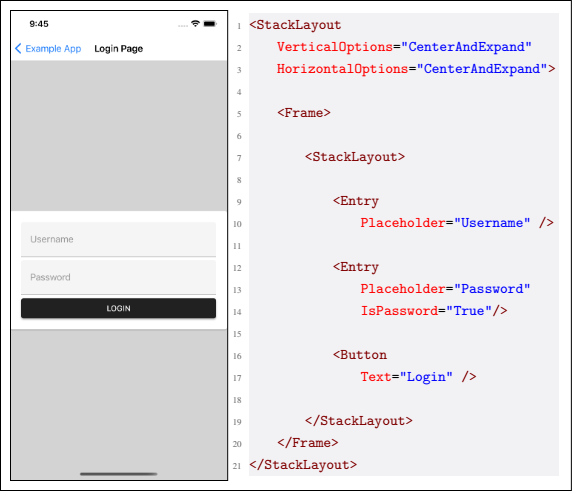
\includegraphics[width=\textwidth,height=\textheight,keepaspectratio]{Images/CrossPlattformFrameworks/ExamplePage.png}
 \caption{Darstellung einer exemplarische Login-Page}
 \label{fig:ExamplePage}
\end{figure}

Mithilfe der Gegenüberstellungen von \ac{ui}-Elementen und Widgets,  kann anschließend eine Transformation des Xamarin.Forms Layout-Baums zu dem Flutter Widget Baum durchgeführt werden.  Zur Verdeutlichung wird in Abbildung \ref{fig:LayoutTrees} eine Baumstruktur verwendet,  welche die Verschachtlung innerhalb der Benutzeroberfläche visualisiert. Das übergeordnete \glq StackLayout\grq{} von Xamarin.Forms sorgt durch \glq CenterAndExpand\grq{}  als Eigenschaftswert für eine zentrierten Darstellung.  In Flutter übernimmt dies das \glq Center\grq{} Widget.  Für alle  Steuerelemente des obigen Quelltextes wird auf in diesem Kapitel verwiesene Widgets zurückgegriffen. 

\begin{figure}[!ht]
 \includegraphics[width=\textwidth,height=\textheight,keepaspectratio]{Images/CrossPlattformFrameworks/Gegenüberstellung.png}
 \caption{Überführung von Xamarin.Forms zu Flutter}
 \label{fig:LayoutTrees}
\end{figure}

Um die Funktionsfähigkeit des Widget-Baums sicherzustellen,  wird er innerhalb einer Flutter-App realisiert, siehe Quelltext \ref{lst:LoginPage}, und das visuelle Ergebnis mit der in Abbildung \ref{fig:ExamplePage} dargestellten Xamarin-Forms App verglichen. 

\lstinputlisting[label={lst:LoginPage},caption={Exemplarische LoginPage in Dart} , language=Dart]{SourceCode/FlutterLoginPage.Dart} 

Bei der Ausführung dieser App fällt auf,  dass visuelle Unterschiede im Vergleich zu der vorher entwickelten Xamarin.Forms Variante existieren.  Im oberen linken Teil der Abbildung \ref{fig:LoginPageFlutter} wird das zentrale Element der Login-Form dargestellt, wobei im Gegensatz zur Xamarin.Forms Variante die Abstände zwischen den Eingabefeldern fehlen.  Außerdem ist der Login-Button nicht über die verfügbare Breite gestreckt.  Abstände die das \glq StackLayout\grq{} automatisch zwischen Elemente legt,  müssen in Flutter durch das \glq Padding\grq{} Widget gesondert nachgestellt werden.  Eine weitere Angleichung ist durch das Widget \glq SizedBox\grq{} durchzuführen,  um die Breite des \glq ElevatedButtons\grq{} anzupassen.  Somit kann der zentrale Bereich des Widget-Baums neu generiert werden,  wie er im unteren Linken Bereich der Abbildung \ref{fig:LoginPageFlutter} veranschaulicht.  Der angepasste Quelltext,  siehe hierzu auch  \hyperref[chap:OptimizedLoginPage]{Anhang II},  erzeugt durch oben genannte Flutter Anpassungen eine Login-Ansicht mit dem im rechten Teil angezeigten \ac{ui} die der Xamarin.Forms Variante sehr nahekommt.

\begin{figure}[!ht]
 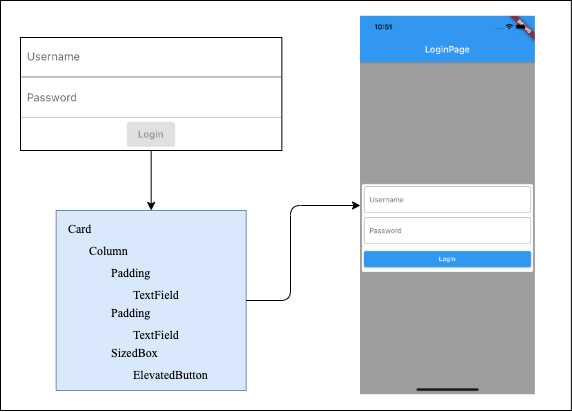
\includegraphics[width=\textwidth,height=\textheight,keepaspectratio]{Images/CrossPlattformFrameworks/FlutterLoginPage.png}
 \caption{Flutter LoginPage Screenshot und Widget-Baum}
 \label{fig:LoginPageFlutter}
\end{figure}

Durch diese Validierung ist ein Beleg für die Annahme,  dass der Austausch von \ac{ui}-Elementen eine App mit vergleichbarer Benutzeroberfläche generieren kann,  erbracht. Jedoch ist für die erfolgreiche Übersetzung von Xamarin.Forms nicht nur die Analyse der Ansichten von elementarer Bedeutung, sondern auch die Berücksichtigung der Eigenschaften und ihrer Kombinationen sowie der nicht im Quelltext ersichtlichen Standartwerte.



  \chapter{Unterschiede zwischen C\# und Dart}
\label{chap:Programmiersprachen}

Nach den in Kapitel \ref{chap:CrossPlattformFrameworks} behandelten Unterschieden zwischen den Frameworks, wird in diesem Kapitel die Heterogenität zwischen den Hochsprachen \Csharp{} und Dart behandelt.  Durch den ähnlichen Stil und vergleichbare Syntax der beiden objektorientierten Programmiersprachen wird der Umstieg von Xamarin.Forms zu Flutter erleichtert.\footcite[Vgl. ][Abgerufen am \today]{Pedley2019}Alle Unterschiede zwischen den Programmiersprachen können innerhalb des Quelltextes der mobilen Anwendung vorkommen und müssen daher bei der Übersetzung von Apps berücksichtigt werden.

\section{Klassendesign}
In diesem Abschnitt sollen die sogenannten Klassen und Objekte der objektorientierten Programmierung betrachtet werden, die sowohl in \Csharp{} als auch in Dart, allerdings mit vereinzelten Unterschieden bei der Realisierung, Verwendung finden. Die sogenannten Objekte werden durch bestimmte,  charakteristische Merkmale beschrieben,  die in der Klassendefinition festgelegt werden müssen. \footcite[Vgl.][S. 11f.]{Witte2013}

\subsection{Referenz- und Wertetypen}
\Csharp{} ist eine Sprache des \glq .NET Frameworks\grq{} und verwendet daher dessen Typ-System,  welches zwischen Werte- und Referenztypen unterscheidet.  Der Unterschied zwischen beiden ist in der Allokation des Systemspeichers zu finden.  Eine Variable des Wertetyps enthält eine Instanz des Typs.  Dies unterscheidet sich von einer Variablen des Referenztyps, der eine Adresse der Speicherzellen des Typs enthält. \footcite[Vgl.][S. 155f.]{Kühnel2019} \Csharp{} bietet die folgenden Wertetypen: Ganzzahlig numerische Typen (Integer),  Fließkomma  Typen (Float und Double),  Wahrheitswerte (Boolean) und ein Zeichen (Char).  Jeder Variablen dieser Typen muss zwingend ein zum Typ passender Wert zugewiesen sein.  Daraus folgt,  dass zu jeder Zeit in einer Instanz des Typs Integer eine Zahl verwaltet werden muss. \footcite[Vgl. ][Abgerufen am \today]{MicrosoftValueTypes2020} Um die Bedingung dieser Wertpflicht zu umgehen,  gibt es in der Hochsprache \Csharp{} die sogenannten \glq nullable\grq{} Typen,  die neben den zulässigen Werten zusätzlich den Wert \glq null\grq{} akzeptieren. \footcite[Vgl.][S. 167]{Bayer2008} 

 
Die Programmiersprache Dart war bis zu der Version 2.12 \glq nicht Null sicher\grq . Da nicht gewährleistet war,  dass Typen einen entsprechenden Wert zu jeder Zeit repräsentieren mussten,  war zur Vermeidung von Laufzeitfehlern eine Nullprüfung, wie in Quelltext \ref{lst:DartNull} dargestellt, bei der Arbeit mit Variablen erforderlich.   

\lstinputlisting[label={lst:DartNull},caption={[Nullsicherheit in Dart bis Version 2.12]{Nullsicherheit in Dart 1.x\footcite[In Anlehnung an ][Abgerufen am \today]{Pedley2019}}}, language=Dart]{SourceCode/DartNull.Dart}

Im März 2021 hat\footcitetext[Quelltext in Anlehnung an][Abgerufen am \today]{Pedley2019} die Programmiersprache Dart den Support für Nullsicherheit hinzugefügt. Diese gravierende Änderung für Softwareentwickler ist in der aktuellen Literatur und vielen Onlineressourcen noch nicht veröffentlicht,  muss jedoch beim Compilerentwurf berücksichtigt werden.  Ab diesem Zeitpunkt ist ein Wert \glq null\grq{} nur noch möglich, wenn der Entwickler dies bewusst entscheidet, ansonsten benötigen Typen einen Wert.  Mit dieser \glq Nullsicherheit\grq{} werden die Laufzeit-Nullreferenzfehler zu Analysefehlern, die während der lexikalischen Analyse auffallen und somit nicht mehr zwangsläufig zum Absturz der Anwendung führen. \footcite[Vgl.][Abgerufen am \today]{GoogleflutterNullSafty2021} Quelltext \ref{lst:DartNotNullAnymore} visualisiert die Arbeit mit den neuen Datentypen in Dart. 

\lstinputlisting[label={lst:DartNotNullAnymore},caption={[Nullsicherheit in Dart 2.12]{Nullsicherheit in Dart 2.x\footcite[In Anlehnung an ][Abgerufen am \today]{GoogleflutterNullSafty2021}}}, language=Dart]{SourceCode/DartNullable.Dart}

Seit \footcitetext[Quelltext in Anlehnung an][Abgerufen am \today]{GoogleflutterNullSafty2021} dieser Veränderung verhält sich die Programmiersprache Dart analog zu \Csharp.  Auch ein Fragezeichen,  das für die Definition eines nullable Typs verwendet wird,  ist identisch.  Spezielle Änderungen sind somit nicht mehr durch den Compiler an dieser Stelle vorzunehmen.  

\subsection{Datentypen}
Die Unterscheidung von Referenz- und Wertetypen ist elementar für die Programmierung mit \Csharp .  Neben den bereits eingeführten Unterschieden bei der Speicherallokation besteht eine weitere Differenz bei der Initialisierung.   Während  Wertetypen einfach der entsprechende Wert zugewiesen werden kann,  muss bei Referenztypen explizit ein Objekt generiert oder ein bestehendes zugewiesen werden.  Die Erzeugung eines neuen Objekts erfolgt durch den Operator \glq new\grq .\footcite[Vgl.][S. 93]{Kofler2005} Dart analysiert, wann ein neues Objekt initiiert werden muss und benötigt daher keinen \glq new\grq{} Operator,  wie in Quelltext \ref{lst:DartNew} dargestellt.  \footcite[Vgl. ][Abgerufen am \today]{GoogleFlutterTour2020} 

\lstinputlisting[label={lst:DartNew},caption={[Objekterzeugung ohne \glq new\grq{} Keyword in Dart]{Objekterzeugung ohne \glq new\grq{} Keyword in Dart\footcite[Quelltext in Anlehnung an][Abgerufen am \today]{Pedley2019}}}, language=Dart]{SourceCode/DartNew.Dart}

Folgend\footcitetext[Quelltext in Anlehnung an][Abgerufen am \today]{Pedley2019}  ist ein Vergleich der eingebauten Datentypen beider Sprachen in Tabelle  \ref{tab:Datatypes} veranschaulicht.

\begin{table}[!ht]
\begin{tabularx}{\textwidth}{|X|X|X|}
\hline

   \textbf{Kategorien} & \textbf{\Csharp{} Datentypen}  &  \textbf{Dart Datentypen}  \\
\hline
	Ganzzahl            			&  sbyte    		& int \\ 
										&	byte 			& 	BigInt			\\ 
										&	short 			& 				\\ 
										&	ushort 			& 				\\ 
										&	int 			& 				\\ 
										&	uint 			& 				\\ 
										&	long 			& 				\\ 
										&	ulong 			& 				\\ 
	\hline
	Fließkommazahl         &  double 			& double \\
										&	float 			& 				\\ 
										&	decimal 			& 				\\ 
	\hline
	Zeichenfolge      					&  string        	& String 					\\ 
	\hline
	Textzeichen      			&  char        	&  					\\ 
	\hline
	Datenfeld      						&  Array        	&  					\\ 
	\hline
	Bool            			& 	bool				& bool \\ 
	\hline
	Auflistung          					& List				& List \\ 
	\hline
	Hashtabelle					& Dictionairy		& Map \\ 
	\hline
\end{tabularx}
\caption{Gegenüberstellung von verfügbaren Datentypen}
 \label{tab:Datatypes}
\end{table}
Es ist ersichtlich,  dass sich einige,  aber nicht alle Datentypen unterscheiden und für manche Typen in Dart eine entsprechende Repräsentation fehlt.  Auf die für den Compilerbau relevanten Unterschiede wird im Folgenden genauer eingegangen. 
\subsubsection{Ganzzahlen}
Wie die Tabelle zeigt,  bietet \Csharp{} eine Vielzahl von Typen für die Arbeit mit Ganzzahlen.  Diese haben einen Bereich von 8 bis 64 Bit und stehen jeweils mit und ohne Vorzeichen zur Verfügung.  Dart besitzt keine vergleichbar umfangreiche Auswahl von Ganzzahl-Datentypen.  Um Zahlen dennoch effizient im Hauptspeicher abzulegen, wird auf unterschiedliche interne Darstellungen zurückgegriffen, je nachdem,  welcher Integer-Wert zur Laufzeit tatsächlich verwendet wird.  Für besonders große Zahlenwerte steht jedoch der DatenTyp \glq Bigint\grq{}  zur Verfügung.  \footcite[Vgl. ][Abgerufen am \today]{Ford2019} Der Compiler muss alle ganzzahligen  \Csharp{} Datentypen zu Dart \glq Integer\grq,  bis auf \glq long\grq{} und \glq ulong\grq{} die von \glq BigInt\grq{}  repräsentiert werden, übersetzten. 

\subsubsection{Fließkommazahlen}


Fließkommazahlen stellen reelle Zahlen dar.  In \Csharp{} stehen dafür, wie in der Tabelle aufgeführt,  verschiedene Datentypen zur Verfügung.  Der \glq decimal\grq -Typ behandelt Dezimalstellen am genauesten,  während die Alternativen \glq double\grq{} und  \glq float\grq{} nur Annäherungen an bestimmte reelle Zahlen erreichen.  \footcite[Vgl. ][Abgerufen am \today]{MicrosoftFlieskomma2021}
In Dart steht für die Arbeit mit Kommazahlen nur der Datentyp \glq  double\grq{} zur Verfügung, \footcite[Vgl. ][Abgerufen am \today]{GoogleDouble} alle Fließkommazahlen müssen daher während der Kompilierung zu \glq double\grq{} umgewandelt werden.

\subsubsection{Textzeichen}

In \Csharp{} sind einzelne Textzeichen ein \glq  Char\grq .  Eine Folge von Textzeichen bildet einen  sogenannten \glq  String\grq.  Dart stellt dagegen keinen Datentyp für einzelne Textzeichen zur Verfügung.  Für eine entsprechende Darstellung wird auf den Datentyp \glq  String\grq{} zurückgegriffen.  Die  \glq String\grq{} Klasse verfügt über einen Konstruktor, der einen \glq CharacterCode\grq{} als Übergabewert erwartet und das String Objekt mit einem  Textzeichen erzeugt. Dies wird in Quelltext \ref{lst:DartStringChar} dargestellt.
\lstinputlisting[label={lst:DartStringChar},caption={Erstellung eines Strings mit einem Zeichen in Dart}, language=Dart]{SourceCode/DartNewStringChar.Dart}


\subsubsection{Datenfelder}

Die vielleicht gebräuchlichsten Datensammlungen sind die sogenannten \glq Arrays\grq{} die auch als Datenfelder bezeichnet werden.  Es sind geordnete Gruppen mit einer festen Anzahl von Objekten eines definierten Typs. \footcite[Vgl.][S. 110f]{Kühnel2019} In Dart gibt es im Vergleich zu \Csharp{} keine \glq Arrays\grq{}.  Alternativ  wird der Datentyp \glq List\grq{}  verwendet,  sodass bei einer Übersetzung von \Csharp{} eine Anpassung der entsprechenden Datentypen erfolgen muss.  Die Arbeit mit Datenfeldern in Dart wird in Quelltext \ref{lst:DartList} dargestellt.
\lstinputlisting[label={lst:DartList},caption={Datenfelder in Dart}, language=Dart]{SourceCode/DartList.Dart}


\subsubsection{Auflistungen}
Anders als die \glq Arrays\grq{}  sind die Auflistungen in \Csharp{} nicht statisch und kontinuierlich sondern dynamisch, was das Einfügen von Elementen vereinfacht.   Diese werden von dem Datentyp \glq List\grq{} repräsentiert,  wie es auch Dart macht.  Der Datentyp \glq List\grq{}  wird in Dart folglich sowohl für Datenfelder als auch für Auflistungen verwendet.

\subsubsection{Hashtabellen}

Eine Hashtabelle ist ein Objekt, das Schlüssel und Werte miteinander verknüpft. Sowohl Schlüssel als auch Werte können beliebige Objekttypen sein.  Jeder Schlüssel darf in einer Hashtabelle nur einmal vorkommen und ist unveränderlich,  während Werte mehrfach verwendet werden können.  
\Csharp{} bietet den Datentyp \glq Dictionary\grq{}  für die Arbeit mit Hashtabellen, in  Dart geschieht dies mittels \glq Map\grq.\footcite[Vgl. ][Abgerufen am \today]{GoogleFlutterTour2020} Im Rahmen der Übersetzung muss der Typ Dictionary folglich durch \glq Map\grq{} ersetzt werden.  Der folgende Quelltext zeigt die Verwendung einer Hashtabelle in der Programmiersprache Dart.
\lstinputlisting[label={lst:DartHashmap},caption={Hashtabellen in Dart}, language=Dart]{SourceCode/DartHashmap.Dart}


\subsection{Modifizierer}

Alle Klassen und Eigenschaften verfügen in beiden Sprachen über eine Zugriffsebene,  die steuert,  ob Objekte von anderem Code verwendet werden können.  Dabei wird in \Csharp{}  mithilfe der Schlüsselwörter \glq public\grq ,  \glq private\grq ,  \glq protected\grq ,  \glq internal\grq ,  \glq protected internal\grq ,  \glq private protected\grq{} der Zugriff geregelt.  In Dart gibt es keine Schlüsselwörter, stattdessen wird mit einem Unterstrich (\_) der Zugriff limitiert.  Im Gegensatz zu \Csharp{} wird der Modifizierer nicht vor dem Datentypen, sondern als Prefix vor dem Membernamen geführt.  Dies wird in Quelltext \ref{lst:PrivatePublicDart}  dargestellt. 

\lstinputlisting[label={lst:PrivatePublicDart},caption={[Private und Public Definitionen in Dart]{Private und Public Definitionen in Dart\footcite[Quelltext in Anlehnung an][Abgerufen am \today]{Pedley2019}}}, language=Dart]{SourceCode/PrivateDefinition.Dart}

Unterstriche  \footcitetext[Quelltext in Anlehnung an][Abgerufen am \today]{Pedley2019} sind erlaubte Zeichen bei der Entwicklung von  \Csharp{} Klassen.  Sie müssen bei der Übersetzung entfernt werden,  da sonst fehlerhafte Übersetzungen drohen.  Durch das Fehlen der anderen oben erwähnten Modifizierer können Berechtigungen in Dart nicht so feingranular definiert werden wie in \Csharp .  Der vom Compiler generierte Dart Quelltext darf nicht mehr Zugriffe verweigern als der ursprüngliche Quelltext,  daher kann es passieren,  dass der Dart Quelltext weniger gute Restriktionen aufweist.  
\subsection{Vererbung}

Erweiterungen oder Veränderung von Klassen entstehen durch die Vererbung, wobei aus einer bestehenden Basisklasse neue abgeleitete Klassen entwickelt werden können, die der Spezialisierung dienen. \footcite[Vgl.  ][Abgerufen am \today]{MicrosoftVeerbung2020}  Der folgende Quelltext zeigt eine Vererbung in Dart.

\lstinputlisting[label={lst:DartInherit},caption={[Vererbung in Dart]{Vererbung in Dart\footcite[Quelltext in Anlehnung an][Abgerufen am \today]{Pedley2019}}},  language=Dart]{SourceCode/DartInherit.Dart}
Einer\footcitetext[Quelltext in Anlehnung an][Abgerufen am \today]{Pedley2019}  abgeleiteten Klasse kann exakt nur eine Basisklasse,  also eine Elternklasse, zugeordnet werden, dies ist bei \Csharp{} und Dart gleich definiert. Eine Mehrfachvererbung ist in \Csharp{} auf Klassenebene nicht vorgesehen, kann aber durch Schnittstellenvererbung erfolgen. Dafür muss eine Implementierung von Attributen oder Methoden über Schnittstellen erfolgen.\footcite[Vgl.][S. 258f.]{Kühnel2019} Dart kennt im Gegensatz zu \Csharp{} keine Schnittstellen,  sondern verwendet stattdessen das Konzept der Mixins.  Auch hier hat jede Klasse genau eine Elternklasse,  jedoch kann ein Klassenkörper in mehreren Hierarchien vorkommen.  Dies wird in Quelltext \ref{lst:DartMixin} visualisiert. 


\lstinputlisting[label={lst:DartMixin},caption={[Mixin's in Dart]{Mixin's in Dart\footcite[Quelltext in Anlehnung an][Abgerufen am \today]{Pedley2019}}}, language=Dart]{SourceCode/DartMixin.Dart}
\footcitetext[Quelltext in Anlehnung an][Abgerufen am \today]{Pedley2019}
\subsection{Übersetzungsbeispiel}
Durch die  herausgearbeiteten Unterschiede in der Klassenmodellierung kann exemplarisch eine  \Csharp{} Klasse zu Dart übersetzt werden,  um einen Eindruck über die Arbeitsweise des Compilers zu vermitteln.  Der folgende Quelltext veranschaulicht die Ausgangsklasse. 

\lstinputlisting[label={lst:CshClass},caption={Beispielklasse in C\#},  language=csh]{SourceCode/ExampleClass.cs}

Dieser Quelltext kann nun zu Dart übersetzt werden,  wie der folgende Quelltextausschnitt demonstriert. 

\lstinputlisting[label={lst:ExampleClassDart},caption={Beispielklasse in Dart}, language=Dart]{SourceCode/ExampleClass.dart}

\section{Namespaces}

Namespaces werden häufig in \Csharp{} Programmen verwendet,  um Klassen zu organisieren.  Die meisten Klassen beginnen mit einem Abschnitt von using-Anweisungen,  der die Namensräume einbindet.  Dadurch können Entwickler auf enthaltene Methoden und Klassen zugreifen, ohne den vollqualifizierten Namen verwenden zu müssen.\footcite[Vgl. ][Abgerufen am \today]{MicrosoftNamespaces2020} 
Dart hat keine Namespaces,  stattdessen werden Pakete und Dateien direkt importiert.  Somit kann ein direkter Zugriff auf alle Klassen und Funktionen innerhalb der Datei gewährt werden.  Im Falle von  Namenskonflikten,  z.B.  gleiche Klassennamen,  können Dateien benannt werden.  Quelltext \ref{lst:DartPackages} zeigt die Arbeit mit Paketen und Dateien in Dart.

\lstinputlisting[label={lst:DartPackages},caption={[Importieren von Paketen in Dart]{Importieren von Paketen in Dart\footcite[[In Anlehnung an ][Abgerufen am \today]{Pedley2019}}}, language=Dart]{SourceCode/DartPackages.Dart}

\section{Generische Typen}
 Generics \footcitetext[Quelltext in Anlehnung an][Abgerufen am \today]{Pedley2019} erlauben es Typen in .NET als Parameter zu übergeben.   Dadurch lassen sich Klassen und Methoden designen,  bei denen ein Typ durch Abstraktion verzögert übermittelt wird.   So kann ein generischer Typparameter eingesetzt werden,  um eine Klasse zu entwickeln, die von unterschiedlichen Methoden verwendet wird,  ohne dass Kosten und Risiken durch Umwandlungsprozesse während der Laufzeit anfallen.\footcite[Vgl. ][Abgerufen am \today]{MicrosoftGenerics2015} 

Generics werden in Dart sehr ähnlich behandelt wie in \Csharp{} allerdings muss keine Typbeschränkung übergeben werden.  \footcite[Vgl.][S. 98]{Cheng2019} Quelltext \ref{lst:DartGeneric} zeigt die Implementation einer generischen State-Klasse in Dart. 

\lstinputlisting[label={lst:DartGeneric}, caption={[Generics in Dart]{Generics in Dart\footcite[Quelltext in Anlehnung an][Abgerufen am \today]{Pedley2019}}}, language=Dart]{SourceCode/DartGeneric.Dart}

\section{Integrierte Verweistypen }
Integrierte Verweistypen (engl. Delegates) \footcitetext[Quelltext in Anlehnung an][Abgerufen am \today]{Pedley2019} referenzieren Methoden mit einer bestimmten Parameterliste und dem Rückgabetyp.  \glq Delegates\grq{} werden dazu verwendet,  Methoden als Parameter zu übergeben.  Im ereignisgesteuerten Framework Xamarin.Forms werden die Methoden zur Behandlung von Ereignissen durch  \glq Delegates\grq{}  aufgerufen.\footcite[Vgl. ][Abgerufen am \today]{MicrosoftDelegates2015} 

In Dart kann der Typ \glq Typedef\grq{} verwendet werden,  um eine Methodensignatur zu definieren und eine Instanz davon in einer Variablen vorzuhalten. \footcite[Vgl. ][Abgerufen am \today]{Pedley2019}  Dies wird in Quelltext \ref{lst:DartDelegates} dargestellt. 

\lstinputlisting[label={lst:DartDelegates},  caption={[Delegates in Dart]{Delegates in Dart\footcite[Quelltext in Anlehnung an][Abgerufen am \today]{Pedley2019}}}, language=Dart]{SourceCode/DartDelegates.Dart}

\section{Asynchronität und Parallelität}

Zur Verbesserung der Leistungsfähigkeit durch Reduktion von Blockierungen wurde das 
aufgabenbasierte asynchrone Programmiermodell bei \Csharp{} eingeführt. 
Bei Synchronität wurde eine Anweisung erst komplett durchgeführt und beendet,  bevor die
Abarbeitung der nächsten begann. Diese strenge Reihenfolge wird durch die Asynchronität 
aufgehoben.  Der Quelltext lässt sich trotz asynchroner Entwicklung weiterhin wie eine Folge von Anweisungen lesen, wird aber in der Praxis möglicherweise in einer deutlich komplizierteren Reihenfolge ausgeführt.\footcite[Vgl. ][Abgerufen am \today]{MicrosoftAsyncAwait2020} 

In Dart wird auf die gleichen Schlüsselwörter \glq async\grq{} und \glq await\grq{}  für die Realisierung von asynchronen Programmen zurückgegriffen.  Dies wird in Quelltext \ref{lst:DartAsync} dargestellt.

\lstinputlisting[label={lst:DartAsync},caption={[Async und Await in Dart]{Async und Await in Dart\footcite[[In Anlehnung an ][Abgerufen am \today]{Pedley2019}}}, language=Dart]{SourceCode/DartAsyncAwait.Dart}

Um\footcitetext[Quelltext in Anlehnung an][Abgerufen am \today]{Pedley2019}  die Vorteile von mehreren Prozessorkernen nutzen zu können,  reicht dieses Konzept jedoch nicht aus.  In Flutter müssen potentielle Hintergrundthreads,  wie in  \Csharp ,  manuell verwaltet werden.  Für den Start von rechenintensiven Arbeiten stehen die \glq Isolates\grq{} zur Verfügung,  die dem Task Konzept aus \Csharp{} ähneln.  Dabei sind \glq Isolates\grq{} separate Ausführungsthreads, die sich keinen Speicher mit dem Hauptspeicher der Anwendung teilen und somit im Gegensatz zu \glq Task\grq{} nicht auf die Anwendung zugreifen können.


\section{Bibliotheken}

Klassenbibliotheken\footcitetext[Quelltext in Anlehnung an][Abgerufen am \today]{Pedley2019} sind das Konzept der freigegebenen Bibliothek für .NET.  Somit können nützliche Funktionalitäten auf Module verteilt und von mehreren Anwendungen verwendet werden.\footcite[Vgl. ][Abgerufen am \today]{MicrosoftClassLibary2016} Dart verfügt über eine Vielzahl von Kernbibliotheken, die für alltägliche Programmieraufgaben, wie das Arbeiten mit Objektsammlungen,  das Durchführen von Berechnungen und das Kodieren sowie Dekodieren von Daten unerlässlich sind.  Zusätzliche \acp{api} sind in von der Community bereitgestellten Paketen verfügbar, die bereits im letzten Kapitel erwähnt wurden. Neben den analogen Konzepten ist auch der Inhalt einiger Bibliotheken vergleichbar.  So ähnelt \glq dart:async\grq{} dem  \glq System.Threading\grq, \glq dart:Math\grq{} dem  \glq System.Math\grq{} und \glq dart.io\grq{} dem \glq System.IO\grq. Eine weitere Besonderheit von Dart ist, dass Funktionalitäten direkt Inhalt von Dateien sein können,  ohne in einer Klasse oder Namespace verschachtelt zu sein. 

\subsection{Netzwerkaufrufe}
Netzwerkaufrufe zur Datenabfrage vom Server oder Übermittlung von Benutzereingaben erfolgt in \Csharp{} durch die Klasse HttpClient,  Dart verwendet das http-Paket.  Um eine Netzwerkanfrage zu stellen,  ist es in beiden Sprachen wichtig, die vorher eingeführten Schlüsselwörter \glq async\grq{} und \glq await\grq{} zu verwenden, damit die Benutzeroberfläche auch während der Anfrage reaktionsfähig bleibt.  Ein Netzwerkanfrage in Flutter wird in Quelltext \ref{lst:FlutterNetworkRequest} dargestellt.

\lstinputlisting[label={lst:FlutterNetworkRequest},caption={Flutter Network request}, language=Dart]{SourceCode/NetworkRequest.Dart}
\subsection{Kodierung und Dekodierung von Daten}

Bei\footcitetext[Quelltext in Anlehnung an][Abgerufen am \today]{Pedley2019}  der Entwicklung von Apps wird häufig \ac{json}, ein kompaktes Format für den Austausch von Daten zwischen Anwendungen, verwendet.  \footcite[Vgl.][S. 684]{Dobrenz2018}  Kodierung,  auch als Serialisierung bezeichnet,  ist die Umwandlung einer Datenstruktur in eine Zeichenkette.  Dekodierung,  auch Deserialisierung, ist der umgekehrte Prozess,  die Umwandlung einer Zeichenkette in eine Datenstruktur. \footcite[Vgl.][Abgerufen am \today]{GoogleJson} In \Csharp{} kann für beide Prozesse der Namespace \glq System.Text.Json\grq{} verwendet werden, \footcite[Vgl.][Abgerufen am \today]{MicrosoftJson2020} während in Dart die Bibliothek \glq dart:convert\grq{} zur Verfügung steht. \footcite[Vgl.][Abgerufen am \today]{GoogleJson}


\section{Ereignisse}
Ein Ereignis ist eine Meldung, die von einem Objekt gesendet wird, um das Auftreten
einer Aktion zu signalisieren. Dies wird beim ereignisgesteuerten Xamarin.Forms z.B. durch den Klick auf eine Schaltfläche ausgelöst. Events können in  \Csharp{}  auch ohne \ac{xaml} Dateien verwendet werden, wenn etwa die Programmlogik das Ändern eines Eigenschaftswerts verursacht.  Das Objekt, von dem das Ereignis ausgelöst wird, ist der Ereignissender, dem die weitere Folge der  Aktion nicht bekannt ist.  Dart verwendet Streams,  die ähnlich wie Ereignisse arbeiten, deren Verwendung in Quelltext  \ref{lst:DartEvents} dargestellt sind.


\lstinputlisting[label={lst:DartEvents},caption={[Events in Dart]{Events in Dart\footcite[[In Anlehnung an ][Abgerufen am \today]{Pedley2019}}}, language=Dart]{SourceCode/DartEvents.Dart}
 \footcitetext[Quelltext in Anlehnung an][Abgerufen am \today]{Pedley2019}



  \chapter{Realisierung des Source-To-Source Compilers}
\label{chap:Realisierung}
Gestützt auf das grundsätzliche Wissen über Compiler, die herausgearbeiteten Unterscheidungen von  Xamarin.Forms und Flutter sowie die Differenzen der verwendeten Programmiersprachen  \Csharp{} und Dart, wird in diesem Kapitel die Realisierung des Source-to-Source Compilers beschrieben.  Es bietet sich die \ac{ide} (deutsch Entwicklungsumgebung) Visual Studio 2019 von Microsoft an,  um das Projekt mit Roslyn Integration zu implementieren,  da auf dieser Plattform Erweiterungen für Roslyn zur Verfügung stehen.
Die zu entwickelnde Projektmappe besteht also aus dem Source-to-Source Compiler mit Rosyln Integration, der grafischen Benutzeroberfläche und einer Xamarin.Forms Anwendung als Testobjekt,  wobei letztere jedoch erst im nächsten Kapitel thematisiert wird.


\section{Programmablauf}
Mithilfe des Roslyn Compilers kann der Source-to-Source Compiler Auswertungen zu den in der Xamarin.Forms App referenzierten Quelltextdateien durchführen.  Somit ist es möglich,  eine Auflistung aller verfügbaren \Csharp-Dateien aus einem Projekt zu extrahieren.  XAML-Dateien werden nicht von Roslyn behandelt.  Dies gelingt jedoch über den Umweg der Codebehind-Dateien mit Endung .XAML.cs,  die ein Laden über das Dateisystem ermöglichen. 

Bevor der Source-to-Source Compiler alle Quelltext- und Ansichtsdateien übersetzt,  müssen die in Kapitel 4 beschriebenen Metadaten überführt werden.  Anschließend kann der Quelltext optimiert und der Übersetzungsvorgang abgeschlossen werden.  Zur Visualisierung des Übersetzungsvorganges dient das in Abbildung \ref{fig:umlablauf} dargestellte \ac{uml}-Aktivitätsdiagramm.

\newpage
\begin{figure}[!ht]
 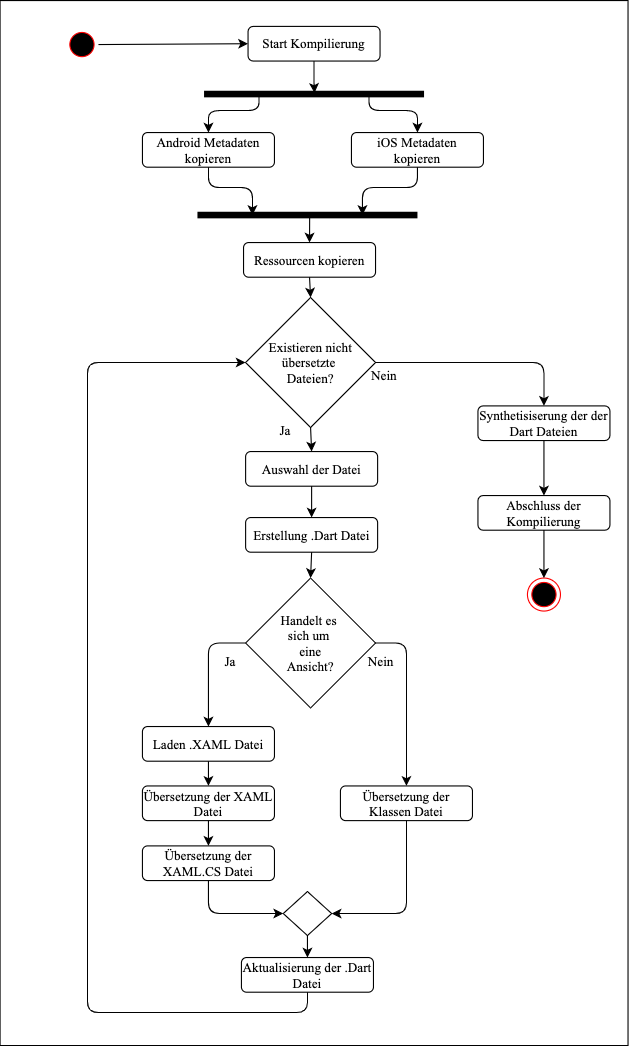
\includegraphics[width=\textwidth,keepaspectratio]{Images/Implementation/Ablauf.png}
 \caption{Aktivitätsdigramm}
 \label{fig:umlablauf}
\end{figure}

Das dargestellte \ac{uml}-Diagramm befindet sich aufgrund der Komplexität des Compilers auf einer hohen Abstraktionsebene. In den folgenden Abschnitten werden die einzelnen Aspekte der Kompilierung noch näher betrachtet.


\section{Metadaten}
Wie das UML Diagramm veranschaulicht, können die Metadaten von Android und iOS parallel in die Flutter Anwendung kopiert werden.  Da die Metadaten
plattformspezifische Eigenschaften der mobilen Anwendungen sind, wird im nächsten Abschnitt auf die entsprechenden Details der beiden Betriebssysteme eingegangen.


\subsection{Android Metadaten}
Zu den Android spezifischen Metadaten gehören die sogenannten Launcher Icons, die den Anwendern als App-Icon angezeigt werden. Xamarin.Android speichert diese grafischen Symbole in Ordnern, die die unterschiedlichen Pixeldichten der Android-Geräte unterstützen und in denen unter Umständen auch andere Bilder gespeichert sind.  Innerhalb von Xamarin.Forms wird das ausgewählte Icon über die Klasse  \glq MainActivity.cs\grq{}  definiert, wie in Quelltext \ref{lst:IconName} dargestellt. 

\lstinputlisting[label={lst:IconName},caption={Xamarin.Forms Android Launcher-Icon Name}, language=csh]{SourceCode/IconName.cs}

Nach der Extraktion des Namens können die entsprechenden Bilder kopiert werden.  In der durch die Flutter SDK erzeugten App liegen bereits Bildplatzhalter für den Austausch bereit.

Der eindeutige Identifizierer,  PackageID,  zählt ebenfalls zu den Metadaten und dient der eindeutigen Erkennung einer Anwendung auf dem mobilen Gerät und im Google Play Store.  Die Information über die PackageID kann in Xamarin.Forms aus der \glq AndroidManifest.xml\grq{} Datei ausgelesen werden und muss in Flutter sowohl in drei Manifest Dateien als auch in die \glq build.gradle\grq{} Konfiguration geschrieben werden.  Das Plugin \glq change\_app\_package\_name\grq{}  nimmt alle notwendigen Änderungen vor.  Es ist als Abhängigkeit zum Projekt hinzuzufügen und anschließend über die Kommandozeile auszuführen. 

Der Anwendungsname wird, wie die PackageID,  aus dem AppManifest extrahiert und in Flutter allerdings nur in eine Manifest Datei im Verzeichnis \glq Project/app/src/main\grq{} geschrieben.  Die Berechtigungen,  die während der Laufzeit der Anwendung beantragt werden,  befinden sich ebenfalls innerhalb des AppManifests und können von hier kopiert werden.

\subsection{iOS Metadaten}
Xamarin.iOS verwaltet die für die Übersetzung notwendigen Metadaten in einer Datei im  Projektverzeichnis mit dem Namen \glq Info.plist\grq .  In Flutter Apps gibt es eine entsprechende Datei,  jedoch werden die Inhalte,  beispielsweise die Bildnummer und der Identifizierer,  aus Variablen geladen.  Damit nach der Kompilierung kein erhöhter Administrationsaufwand bei der Verwaltung dieser Eigenschaften entsteht,  soll dieses Schema beibehalten werden.  Die \glq AppFrameworkInfo.plist\grq{} stellt die Quelle aller Werte,  die als Variablen in die \glq Info.plist\grq, geladen werden müssen dar.   Daher werden die entsprechenden Einträge aus der \glq Info.plist\grq{} von Xamarin.Forms extrahiert und jeweils in die entsprechenden \glq Info.plist\grq{} Dateien von Flutter kopiert.  Tabelle \ref{tab:InfoPlist} zeigt die Zieldatei für die Kopie bestimmter Werte.

\begin{table}[!ht]
  \begin{tabularx}{\linewidth}{|l|X|X|}
  \hline

  \textbf{Schlüssel}  &  \textbf{Info.plist} & \textbf{AppFrameworkInfo.plist} \\
\hline
  DevelopmentRegion  		&  					& 		\checkmark	 \\
  ShortVersionString  		&  					& 		\checkmark	 \\
  Version  							&  					& 		\checkmark	 \\
  MinimumOSVersion  		&  					& 		\checkmark	 \\
  
  InterfaceOrientations  		& \checkmark  	&		 					\\
  BundleSignature  			&  \checkmark 	& 							\\
  BundleName  					&  \checkmark 	& 		 					\\
  \hline
\end{tabularx}
\caption{Info.plist Einträge in Flutter}
 \label{tab:InfoPlist}
\end{table}
Die Übersicht weist nicht alle aus der iOS Entwicklung bekannten Schlüssel auf.  Alle fehlenden Eigenschaften gehören in die Datei \glq Info.plist\grq, wie die letzten drei in der Tabelle \ref{tab:InfoPlist} genannten.  Ähnlich dem Vorgehen bei den Android Metadaten kann für die Modifizierung  von Anwendungsnamen und Identifizierer auf iOS eine Erweiterung verwendet werden.  So kann der Compiler das \glq rename\grq{} Plugin verwenden und es bedarf keiner zusätzlichen manuellen Entwicklung. \footcite[Vgl.][Abgerufen am \today]{Rename}  Die aus iOS bekannten Texte,  zur Beantragung von Berechtigungen müssen weiterhin vom Source-To-Source Compiler extrahiert und in die Flutter \glq info.plist\grq{} transferiert werden.

Für das Anwendungsicon kann das Verzeichnis \glq Assets.xcassets\grq{} aus dem Stammverzeichnis der Xamarin.Forms iOS App in das Verzeichnis \glq ios/flutter/Runner\grq , das alle notwendigen Bilder enthält,  kopiert werden. 

\section{Ressourcen}

Neben den Metadaten ist die Ressourcenkopie der mobilen Anwendung vonnöten.  Dazu gehören die innerhalb der App angezeigten Bilder, die bei Xamarin.Forms üblicherweise innerhalb der plattformspezifischen Anwendungen abgelegt sind. Von dort aus kopiert der Compiler die Bilder aus dem iOS Projekt in das Flutter Projekt zur späteren Verwendung.  Da für Bilder im Flutter Framework keine plattformspezifische Unterscheidung vorgesehen ist,  werden ausschließlich die Bilder aus der iOS App entnommen.  Eine Entscheidung zugunsten der iOS Alternativen wurde  getroffen,  da sich die Konzepte von Xamarin.iOS und Flutter im Bezug auf Bilderressourcen ähneln und eine automatisierte Überführung möglich ist.  Android spezifische Varianten werden während der Übersetzung also nicht berücksichtigt.   
Zur Speicherung und Darstellung höher aufgelöster Bilder existieren zwei Unterordner mit den Namen  \glq 2.0x\grq{} und  \glq 3.0x\grq{} im Verzeichnis Assets.  Ressourcen werden je nach Skalierungsfaktor  \glq @2x\grq{} oder  \glq @3x\grq{} in den entsprechenden Verzeichnissen und ohne Option im Ordner Asset abgelegt.
Neben dem differenzierten Vorgehen bei der Kopie ist es erforderlich,  die Ressourcen in der \glq pubspec.yaml\grq{} zu referenzieren.  Ein Ausschnitt aus der \glq pubspec.yaml\grq ,  der das Einbinden von Bildern demonstriert,  wird in Quelltext \ref{lst:RefImage} dargestellt.

\lstinputlisting[label={lst:RefImage},caption={Referenzierung von Bildern in der pubspec.yaml}, language=Dart]{SourceCode/FlutterPubspecImage.pub} 


Benutzerdefinierte Schriftsätze müssen ebenfalls aus dem iOS Verzeichnis kopiert und anschließend in der \glq pubspec.yaml\grq Datei hinzugefügt werden.  Hier gilt,  analog zu den Bildern,  dass die kompilierte Flutter Anwendung ausschließlich die Schrift der iOS App verwendet und androidspezifische Schriftsätze verloren gehen.

Weitere Ressourcen bilden die Startbildschirme der verschiedenen Plattformen,  die während des Ladens der App angezeigt werden und für eine Veröffentlichung im Appstore verpflichtend sind.  Durch ihren simplen Aufbau entsteht keine zusätzliche Ladezeit und ihr Quelltext wird plattformspezifisch realisiert.  Der Compiler verarbeitet ausschließlich einzelne Bilder, die während des Ladens der mobilen Anwendung angezeigt werden und verzichtet auf die Übersetzung des plattformspezischen Programmcodes,  wie in den Ausschlusskriterien erwähnt.  Da die Xamarin.Forms App nicht zwangsläufig ein Bild in einem entsprechenden Format vorhält,  greift der Flutter Startbildschirm auf das LauncherIcon der jeweiligen Plattformen zurück.  

\section{Übersetzung von Klassenstrukturen}

Die Übersetzung von \Csharp{} zu Dart ist ein essentieller Bestandteil des Compilers.  Dafür wird zuerst die Visual Studio Projektmappe geladen.  Anschließend kann fokussiert das Projekt betrachtet werden, welches den plattformunabhängigen Quelltext beinhaltet.  Da dieser selbst, wie bereits in den Ausschlusskriterien erwähnt,  unübersetzt bleibt, sind die entsprechenden Projekte ausschließlich für das Kopieren der Metadaten und Ressourcen notwendig.  Alle Klasse durchlaufen die in Quelltext \ref{lst:CsharpFrontend} dargestellten Ausführungsschritte. 
\lstinputlisting[label={lst:CsharpFrontend},caption={C\# Compiler Frontend}, language=csh]{SourceCode/CompilerFrontEnd.cs}
Für die Übersetzung von einer Programmiersprache zu einer anderen ist es notwendig,  alle Knoten und Token innerhalb eines Syntaxbaums in der richtigen Reihenfolge zu betrachten.  Die abstrakte Klasse \glq CSharpSyntaxWalker\grq{} erlaubt es,  einen eigenen \glq Syntax-Walker\grq{} zu konstruieren,  der die Knoten und Token analysiert.  Dafür kann von \glq CSharpSyntaxWalker\grq{} geerbt und folgend die \glq Visit()\grq{} Methode überschrieben werden.  \footcite[Vgl.][Abgerufen am \today]{Varty2014}  Der Quelltext \ref{lst:CsharpFrontend} visualisiert die Erstellung eines \glq FlutterTranspilerVisitors\grq ,  mithilfe des vorher ermittelten semantischen Models.  Nun wird der ausgelesene Wurzelknoten des Syntaxbaumes als Parameter der \glq Run()\grq{} Methode übergeben,  die den \glq Visitor\grq{} startet.  

Hiermit endet das Compiler Frontend und es beginnt die Konstruktion des Dart Programmcodes.  Dafür werden die einzelnen Knoten des Baumes je nach ihrem Typen zu entsprechenden Dart Synonymen umgewandelt und die einzelnen Methoden des \glq CSharpSyntaxVisitor\grq{} überschrieben.  Quelltext \ref{lst:PropertyDeclaration} zeigt die Umwandlung von Eigenschaftsdeklarationen.
\newpage
\lstinputlisting[label={lst:PropertyDeclaration},caption={Compilierung von Eigenschaftsdeklarationen}, language=csh]{SourceCode/Modifizierer.cs}

Der Quelltextausschnitt veranschaulicht die generelle Arbeitsweise des Compilers,  der einzelne Zeichen und Zeilen des Dart-Textdokumentes generiert und speichert.  So hangelt sich der Compiler durch das Dokument und übersetzt den Quelltext Schritt für Schritt, wobei die Reihenfolge, in der der Typ, der Zugriffsmodifizierer und der Name der Eigenschaft in die Dart Datei geschrieben wird,  von entscheidender Bedeutung ist.  Die Quelltextzeilen 6 bis 8 geben zuerst den Eigenschaftstyp,  gefolgt von dem optionalen Zugriffsmodifizierer und dem Namen aus.  Zusätzlich kann nun ein Wert gesetzt werden,  bevor ein Semikolon die Deklaration beendet.  Die Methode für die Generierung des Dart Modifizierers zeigt Quelltext \ref{lst:DartModifier}.


\lstinputlisting[label={lst:DartModifier},caption={Austausch von C\# Zugriffsmodifizierern}, language=csh]{SourceCode/Modifier.cs}

Wie bereits in Kapitel 5 beschrieben,  sind die Typen der beiden Programmiersprachen nicht identisch und müssen daher entsprechend angepasst werden.  Zur Veranschaulichung wird die realisierte Methode in Quelltext \ref{lst:DataType} dargestellt. 
\lstinputlisting[label={lst:DataType},caption={Austausch von C\# Datentypen}, language=csh]{SourceCode/Datatypes.cs}

Der Rückgabewert dieser Methode ist der entsprechende Dart Datentyp.  Sollte keine entsprechende Repräsentation verfügbar sein,  erfolgt die Rückgabe des ursprünglichen Typnamens.  Dies ist notwendig,  um andere übersetzte Klassen im Quelltext verwenden zu können.  Damit keine unerwünschten Typen des .Net Frameworks oder von Xamarin.Forms Erweiterungen innerhalb des Übersetzungsergebnisses erscheinen, sind Bereinigungen erforderlich. 

Erweiterungen ergänzen die Funktionalität der Frameworks,  sind jedoch herstellerabhängig mit unterschiedlichen Anforderungen programmiert,  sodass es für Klassen und Methoden aus diesen Bibliotheken nicht zwangsläufig identische Repräsentationen gibt.  Eine Auflösung der Inkompatibilität ist nicht mittels Automation möglich, sondern bedarf unterschiedlich umfangreicher manueller Umwandlungen.  Der Komplexität ist es geschuldet,  dass der Compiler nur eine Auswahl von Erweiterungen unterstützt.  Nachträgliche Erweiterungen des Funktionsumfanges sind möglich.  Die folgenden Anwendungsfälle skizzieren das Vorgehen.  

Mobile Anwendungen nutzen Bilder, die neu über die Kamera aufgenommen werden oder aus der bestehenden Galerie stammen.  Im folgenden wird der Quelltext dargestellt, der die Funktionalität des Xamarin.Forms Essentials mit dem Flutter Plugin \glq image\_picker\grq{} austauscht.  Die notwendigen Berechtigungen wurden bereits während der Übernahme der Metadaten gesetzt und können daher an dieser Stelle ignoriert werden.

\lstinputlisting[label={lst:MediaPlugin},caption={Austausch der Kamera und Galerie Erweiterung}, language=csh]{SourceCode/ImagePluginSwap.cs}

Ein weiterer wichtiger Anwendungsfall,  der nur mithilfe von Erweiterungen implementiert werden kann,  ist der Zugriff auf die Smartphone Sensoren.  Der folgende Quelltext zeigt den Austausch der Beschleunigungssensorfunktionen des Xamarin.Essentials Plugins mithilfe des Flutter Sensor Plugins.  Der Compiler übersetzt ebenfalls die Funktionalität des Gyroskops, siehe Programmcode \ref{lst:Sensor},  da der Quelltext jedoch analog ist, wird er an dieser Stelle nicht explizit aufgeführt. 

\lstinputlisting[label={lst:Sensor},caption={Austausch der Beschleunigungssensor Erweiterung}, language=csh]{SourceCode/Accelerometer.cs}

 Obwohl es keine Gewährleistung gibt, dass für jede Xamarin Forms eine entsprechende Flutter 
Erweiterung zur Verfügung steht, konnte bei der Implementierung des Compilers immer eine  Alternative gefunden werden.


\section{Übersetzung von Ansichten}
Xamarin.Forms Ansichten bestehen, wie bereits beschrieben,  aus den XAML und XAML.CS Dateien, die nach der jeweiligen Übersetzung  in einer gemeinsamen Dart Datei synthetisiert werden.  
Die Kompilierung der beiden Dateien geschieht jeweils durch ein dediziertes Compiler Frontend, das die Aufgaben bis zur Zwischendarstellung übernimmt.  Darauf aufbauend wird ein gemeinsames Compiler-Backend für die Zusammenführung und die Code-Optimierung entwickelt.  Die Abbildung  \ref{fig:ViewCompilerPhases} veranschaulicht den Vorgang. 

\begin{figure}[!ht]
 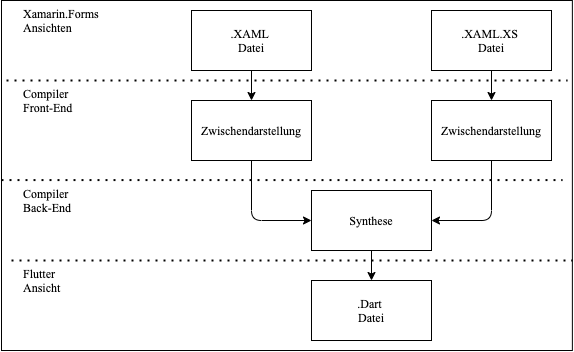
\includegraphics[width=\textwidth,keepaspectratio]{Images/Implementation/ViewCompiler.png}
 \caption{Compiler Phasen für Ansichten}
 \label{fig:ViewCompilerPhases}
\end{figure}

\subsection{Visuelle- Zwischendarstellung}

Für die visuelle Zwischendarstellung wird in einem ersten Schritt die XML Struktur
aus der XAML Datei ausgelesen und als Syntaxbaum interpretiert.  Er beinhaltet eine Auflistung von untergeordneten Elementen,  die weitere Elemente beinhalten können,  sodass eine Verschachtelung  entsteht.  Jedes Element besitzt eine Auflistung von Eigenschaften, die Attribute der einzelnen XML Knoten beschreiben.  Die baumartige Struktur des Xamarin.Forms Layouts wird durch die in Kapitel 4 beschriebenen Repräsentationen von Flutter Widgets in einen Flutter Widget-Baum überführt und für jedes Widget der Quelltext zur Initialisierung in einem Template vorgehalten.  Alle Eigenschaften besitzen in dieser Vorlage vorgefertigte Platzhalter, wie in Quelltext \ref{lst:Placeholder} dargestellt.

\lstinputlisting[label={lst:Placeholder},caption={Vorlage eines Flutter Text-Widgets} , language=Dart]{SourceCode/DartPlaceholder.dart} 

Aufgrund von Inkompatibilitäten zwischen den von Xamarin.Forms gelieferten und von Flutter erwarteten Eigenschaftswerten, ist es notwendig diese umzuwandeln.  Der folgende Quelltext \ref{lst:Parsing} zeigt die Modifizierung von Textgrößen.  Xamarin.Forms fordert den Wert entweder als Zahl oder als sogenannte benannte Größe,  wie \glq Large\grq{} oder \glq Title\grq , während Flutter ausschließlich Textgrößen mit dem Typen Double akzeptiert.   

\lstinputlisting[label={lst:Parsing},caption={Umwandlung von Schriftgrößen} , language=csh]{SourceCode/CSharpFontSize.cs} 

Mittels vergleichbarer Implementierung sind auch an anderen Eigenschaften,  wie z.B. Farbwahl oder Textumbruchoptionen,  Anpassungen erforderlich.

Nun erfolgt die Anlage einer Arbeitskopie des Templates,  um in weiteren Compilerphasen die Werte aus der Xamarin.Forms App einzufügen.  Abbildung \ref{fig:PlaceholderOptions} visualisiert die Behandlung der Platzhalter in den einzelnen Phasen der Übersetzung.


\begin{figure}[!ht]
 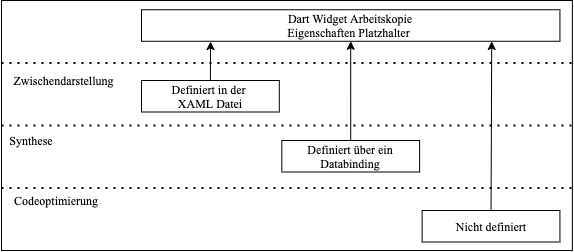
\includegraphics[width=\textwidth,keepaspectratio]{Images/Implementation/DartPlaceHolder.png}
 \caption{Bereinigung von Dart Widget Platzhaltern}
 \label{fig:PlaceholderOptions}
\end{figure}

Es wird deutlich, dass in der Zwischendarstellung ausschließlich XAML definierte Eigenschaftswerte 
importiert werden.  Während der Synthese erfolgt der Austausch der sogenannten Databindings, die den Wert aus der Codebehind-Datei erhalten.  Zur Übersetzung werden neue Platzhalter mit dem Prefix \glq BindingPlaceholder\grq{} benötigt,  die in der Arbeitskopie hinterlegt sein müssen. Exemplarisch wird in Quelltext  \ref{lst:PlaceholderBinding} der Text-Platzhalter zu einem Binding Platzhalter umgewandelt, und der Platzhalter textAlign mit einem Wert versehen. 

\lstinputlisting[label={lst:PlaceholderBinding},caption={Flutter Widget mit Binding-Platzhaltern} , language=Dart]{SourceCode/DartPlaceholderBinding.dart} 

Zu diesem Zeitpunkt sind in der Arbeitskopie noch die Binding- und die ungenutzten Platzhalter vorhanden.  Diese müssen, wie in der Abbildung \ref{fig:PlaceholderOptions} visualisiert,  in späteren Phasen der Kompilierung entfernt werden.  Grundsätzlich lässt sich aus der XAML Datei ableiten,  welche Platzhalter nicht benötigt werden.  Da die Bereinigung jedoch eine Teilaufgabe der Optimierung darstellt, wird sie erst in der entsprechenden Phase im Compiler-Backend durchgeführt. 

\subsection{Logische Zwischendarstellung}

Die Erzeugung der logischen Zwischendarstellung,  basierend auf den Codebehind Dateien,  erfordert die gleiche Implementierung mit \glq CSharpSyntaxWalker\grq{} wie die der Klassenstrukturen,  da es sich bei diesen Dateien ebenfalls um \Csharp{} Klassen handelt.  

Xamarin.Forms übermittelt Änderungen an  Eigenschaften automatisch, mithilfe der \glq INotifyPropertyChanged\grq{}  Schnittstelle, an die Benutzeroberfläche.  Bei Flutter erhält das Framework durch die \glq setState\grq{}  Methode entsprechende Informationen.  Der Compiler kann notwendige Änderungen nicht im Rahmen der Zwischendarstellung durchführen, da anhand der Codebehind Dateien nicht identifizierbar ist, welche Eigenschaften einen direkten Bezug auf die graphische Benutzeroberfläche haben. 

\subsection{Visuelle Synthese}

Die Zusammenführung der visuellen und logischen Zwischendarstellung erfolgt während der visuellen Synthese im Compiler-Backend.  In einem ersten Schritt erfolgt die Kopie der übersetzten Logik unterhalb der für den Aufbau der grafischen Benutzeroberfläche beinhalteten \glq Build\grq{} Methode.  Im nächsten Schritt werden ereignisauslösende Aktivitäten,  beispielsweise der Klick auf Schaltflächen wie in Quelltext \ref{lst:Synth} dargestellt,  mit den übersetzten Methoden verbunden und die Platzhalter entfernt.  Dabei wird der Name der behandelten Methode aus der XML Struktur extrahiert und der entsprechende Binding-Platzhalter mit dem Namen und dem Parameter \glq Context\grq{} ersetzt. 


\lstinputlisting[label={lst:Synth},caption={Synthese von ereignisauslösenden Aktivitäten} , language=csh]{SourceCode/ClickSynth.cs} 

Die Sicherstellung der automatischen Aktualisierung der Benutzeroberfläche kann an dieser Stelle durch die Verwendung von SetState-Blöcken realisiert werden.  Dafür wird der Eigenschaftsname aus dem Binding-Platzhalter extrahiert und im Quelltext überprüft, wo die entsprechende Eigenschaft manipuliert wird.  Die ermittelten Zeilen werden anschließend mit einem SetState-Block eingeschlossen.


\section{Referenzierung}
Im Anschluss an die Zwischendarstellung, in der die Generierung von Logik und Ansichten erfolgte,  müssen nun die entstandenen Dartartefakte untereinander referenziert werden.  Darunter wird in diesem Zusammenhang die Verknüpfung der entsprechenden Quelltextdokumente verstanden.  Diese Verlinkung ist erforderlich,  damit Komponenten auf Klassen zugreifen können,  die in anderen Dateien definiert sind.  Im Gegensatz zu \Csharp{} können Dateien in Dart nicht über Namespaces, sondern nur über ihren Dateinamen eingebunden werden.  Folglich ist es erforderlich,  Dateien in Quelltextdokumente einzubinden,  die verwendete Klassendefinition enthalten.  Die Information,  in welcher Datei sich eine Klasse befindet, wurde durch den \glq CSharpSyntaxWalker\grq{} festgehalten.  Diese Referenzen werden ebenfalls benötigt,  um durch die Anwendung zu den Navigationszielen zu gelangen, da es sich bei der Navigation um die Erzeugung eines Objektes des entsprechenden Widgets handelt. 


\section{Codeoptimierung}

Nach der erfolgreichen Zusammenführung der einzelnen Artefakte kann der Code optimiert werden. Dafür werden Sprachkomponenten einschließlich der Ereignisdefinition,  der Ereignishandler und aller Aufrufe entfernt, die  nur für die  Arbeit von Xamarin.Forms benötigt  wurden. Die Löschung betrifft die \glq InitializeComponent\grq{}  Methode, die aus der Codebehind-Datei die grafische Benutzeroberfläche geladen hat und die bereits durch SetState-Blöcke ersetzte
 \glq INotifyPropertyChanged\grq{}  Schnittstellen Definition,  die für die Oberflächenaktualisierung zuständig war.  Jetzt folgt die Entfernung der nicht benötigten Platzhalter mit dem in Quelltext \ref{lst:PlaceholderCleanup} dargestellten Algorithmus,  aus dem generierten Dart Quelltext.  
\lstinputlisting[label={lst:PlaceholderCleanup},caption={Bereinigung von ungenutzten Platzhaltern}, language=csh]{SourceCode/Cleanup.cs}
Damit befindet sich der Programmcode in einem korrekten syntaktischen Zustand und kann mithilfe des Flutter Compilers zu einer mobilen App übersetzt und ausgeführt werden.  Es wird jedoch noch ein weiterer Schritt in der Codeoptimierung durchgeführt,  der die Lesbarkeit des Quelltextes durch eine einheitliche Formatierung verbessert.  Durch die Verwendung der Templates ist der generierte  Widget-Baum innerhalb der Build Methode nicht eingerückt.  Die Flutter SDK bietet jedoch die Möglichkeit,  Quelltext-Dokumente über die Kommandozeilen Schnittstelle zu formatieren.  Quelltext \ref{lst:Formatting} zeigt die Methode zur Quelltextformatierung mithilfe der Flutter SDK. 

\lstinputlisting[label={lst:Formatting},caption={Methode zur Quelltextformatierung} , language=csh]{SourceCode/FlutterFormatting.cs} 


\section{Grafische Benutzeroberfläche}
Die \ac{gui} ist der zentrale Berührungspunkt von Anwendern mit dem Transpiler.  Sie soll die notwendigen Eingabemöglichkeiten anbieten, das Ergebnis ausgeben und den Anwender auf mögliche Fehler hinweisen.  Das grafische Vorbild ist das in Kapitel 3 entworfene Mockup, siehe Abbildung 3.4.  Für die Erstellung einer entsprechenden Benutzeroberfläche stehen eine Vielzahl von Technologien mit verschiedenen Vor- und Nachteilen zur Verfügung.  Eine Webseite erspart dem Anwender einen hohen Installationsaufwand und ermöglicht die plattformunabhängige Verwendung des Compilers.  Allerdings ist zumindest ein gewisser Kontrollverlust über den eigenen Quelltext durch das  Hochladen auf eine Webseite nicht ausgeschlossen.  Die Bedienoberfläche dieser Arbeit soll daher eine lokale Anwendung sein, sodass kein  unberechtigter Zugriff auf den Source-Code möglich ist.  Zu diesem Zweck wird die \ac{gui}  mit der Technologie \ac{wpf} realisiert.  Dabei handelt es sich um ein UI-Framework des .NET Frameworks, das für die Erstellung von mit XAML und \Csharp{} entwickelten Desktopanwendungen geeignet ist. \footcite[Vgl.][S. 1f]{Wenger2012} 

Anwendungen,  die mittels WPF programmiert werden, sind nur unter Windows als Betriebssystem ausführbar.  Da der Roslyn Compiler auch nur unter Windows verfügbar ist,  entstehen hier keine zusätzlichen Einschränkungen.  Die folgende Darstellung \ref{fig:CompilerUI} zeigt das Erscheinungsbild der Anwendung nach einer erfolgreichen Übersetzung.
\newpage
\begin{figure}[!ht]
 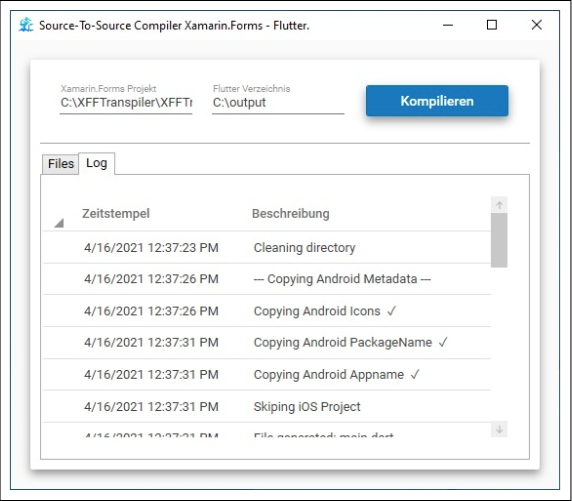
\includegraphics[width=\textwidth,keepaspectratio]{Images/Implementation/UiScreenshot.png}
 \caption{Grafische Oberfläche des Compilers}
 \label{fig:CompilerUI}
\end{figure}

Wie die Ansicht veranschaulicht, werden die durchgeführten Arbeitsschritte durch Log-Einträge in der Anwendung angezeigt.
Die Realisierung der grafischen Benutzeroberfläche 
und des Source-To-Source Compilers erfolgte mit  .Net Technologien,  sodass es möglich ist,  den Compiler als Abhängigkeit in das Projekt der grafischen Benutzeroberfläche zu laden und von dort aus die Übersetzung zu starten.  Eine vollständige Anleitung für die Installation der \ac{gui}  befindet sich in  \hyperref[chap:Installationsanleitung]{Anhang V}.
  \include{07Qualitätssicherung}
  \chapter{Fazit}
\label{chap:FazitAusblick}
Ein Source-To-Source Compiler,  wie in dieser Arbeit entwickelt, stellt einen Lösungsansatz für Xamarin.Forms App-Entwickler dar,  die sich nach dem Ende des Supports vom Anbieter Microsoft trennen und trotzdem eine bestehende Anwendung erhalten möchten.  Das generelle Problem der Abhängigkeit ist jedoch nicht durch eine Abwendung von Microsoft gelöst, da das von der Firma Google entwickelte Flutter Framework ebenfalls, wenn auch derzeit nicht absehbar,  eingestellt werden könnte.  Die Idee durch automatisierte Übersetzungen Programmierern eine Wahlfreiheit und Wechseloptionen zu ermöglichen rechtfertigt eine Weiterentwicklung des Prototypen.

\section{Open Source Veröffentlichung}

Der Umfang des Prototypen wurde durch die in Kapitel \ref{chap:CompilerEntwurf} ausgeschlossenen Aspekte reduziert,  da diese für die Beantwortung der Forschungsfrage eine untergeordnete Rolle spielen.  Diese Einschränkungen besteht bei den meisten Xamerin.Forms Apps nicht.  
Eine Veröffentlichung des Compilers als Open Source Projekt könnte helfen, diese komplexeren 
mobilen Anwendungen zu übersetzen,  indem Programmierer den dann für die Allgemeinheit verfügbaren Quelltext auf spezielle Gegebenheiten anpassen und wiederum publizieren.  
Unternehmen wie DevExpress,  Syncfusion und Telerik bieten sowohl Steuerelemente für 
Xamarin.Forms,  als auch Widgets für Flutter und hätten die Möglichkeit ihre eigenen \ac{ui}-Elemente 
durch den Compiler ersetzten zu lassen und somit dessen Umfang zu erhöhen.  Die Open-Source Lizenz GPL 3.0 würde garantieren,  das Veränderungen am Source-To-Source Compuler wiederum Quelloffen zu seien haben.  Durch die Open Source Veröffentlichung könnte also die Compilerentwicklung in Geschwindigkeit und Zielgenauigkeit erhöht werden.

\section{Beantwortung der Forschungsfrage}
Es besteht die Möglichkeit Apps von Xamarin.Forms zu Flutter vollautomatisiert, ohne manuelle 
Arbeitsschritte zu übersetzten. Zwar überträgt der Source-To-Source Compiler die Xamarin.Forms Testapp und zeigt damit die Machbarkeit einer automatisierten Transformation,  damit jedoch auch produktive Anwendungen vollständig, inklusive plattformspezifischer Implementierungen oder 
anwendungsspezifischer Erweiterungen, ohne manuelles Zutun übersetzt werden können,  sind 
Weiterentwicklungen beispielsweise durch eine Open-Source Veröffentlichung nötig.
Im aktuellen Zustand ist der Compiler schon in der Lage komplexe visuelle Darstellungen
und Quelltexte zu übersetzen und somit den Entwicklungsaufwand bei einem Umstieg auf Flutter 
merklich zu reduzieren.
Kritisch angemerkt sei,  dass manuelle Arbeitsschritte bei der Übersetzung notwendig werden,  sobald eines der ausgeschlossenen Aspekte verwendet wird.


\section{Ausblick}
Bereits für Ende 2021 ist das Supportende für Xamarin.Forms beschlossen und die Einführung von 
.NET \ac{maui} angekündigt.  Eine vollständige Funktionsfähigkeit des Compilers wäre noch in diesem Jahr wünschenswert,  um Unternehmen und Programmierern eine rechtzeitige Alternative zu bieten. 

Anwendungsentwickler bekommen durch den Umstieg von Xamarin.Forms zu Flutter seit März 2021 die Möglichkeit ihre Anwendung als Webseite zu veröffentlichen und somit eine weitere Plattform zu nutzen.  Jedoch sind zusätzliche Implementierungen in der Flutter App notwendig um die Webdarstellung auf großen Displays zu optimieren.  Flutter treibt seine Frameworkentwicklung durch Neuerungen, wie den Support der Webnutzung,  weiter voran,  sodass derzeit nicht der 
Eindruck entsteht, dass ein Supportende in naher Zukunft zu befürchten ist. 
Ob die Einführung von .Net \ac{maui} wegweisende Innovationen mit sich bringt,  ist bisher genau so unbekannt wie der Programmieraufwand für den Umstieg von Xamarin.Forms.  
Der Source-To-Source Compiler stellt daher eine berechenbare Alternative zum Umstieg auf .NET  \ac{maui} zur Verfügung. 

  
  \appendix                       % Leitet den Nachspann ein
  
    \renewcommand*\chapterheadstartvskip{}% removes space before chapter titles 

  \renewcommand*{\chapterpagestyle}{scrheadings}

\setlength\bibitemsep{1.5\itemsep}
\chapter*{Literaturverzeichnis}
 \chaptermark{Literaturverzeichnis}

 \addcontentsline{toc}{chapter}{Literaturverzeichnis}

\printbibliography[nottype=online, heading=subbibliography, title={Gedruckte Quellen}]
\printbibliography[type=online, heading=subbibliography, title={Online Quellen}]
  \include{AnhangGegenüberstellung}
  \chapter{Anhang II: Optimierte Flutter-LoginPage}

\lstinputlisting[label={lst:LoginPage20},caption={Exemplarische LoginPage in Dart} , language=Dart]{SourceCode/FlutterLoginPageUpdate.Dart} 

 % \chapter{Anhang II: Testfälle für den Compiler}
\label{chap:Testfälle}

\begin{xltabular}{\textwidth}{l|X|l}
   \textbf{ID} & \textbf{Beschreibung} & \textbf{Status}  \\  
\hline

	1             			& 			Das Icon der Anwendung wird sowohl für Android als auch für iOS übernommen       &  \checkmark   	\\ 
	2             			& 			Der Name der Anwendung wird sowohl für Android als auch für iOS übernommen       &  \checkmark   	\\ 

	3            			& 			FlyOutPage wird zu MasterDetailScaffold übersetzt      &  \checkmark   	\\ 
	4            			& 			NavigationPage wird zu Scaffold übersetzt      &  \checkmark   	\\ 
	5            			& 			TabbedPage wird zu TabBar und TabBarView übersetzt      &  \checkmark   	\\ 
	
	
	6            			& 			AbsolutLayout wird zu Positioned übersetzt      &  \checkmark   	\\ 
	7            			& 			ContentView wird zu StatelessWidget übersetzt      &  \checkmark   	\\ 
	8            			& 			Frame wird zu BoxDecoration übersetzt      &  \checkmark   	\\ 
	9            			& 			Grid wird zu GridView übersetzt      &  \checkmark   	\\ 
	10            			& 			ScrollView wird zu SingleChildScrollView übersetzt      &  \checkmark   	\\ 
	11           			& 			StackLayout wird zu Row und Column übersetzt     &  \checkmark   	\\ 
	12            			& 			RelativLayout wird zu Positioned übersetzt      &  \checkmark   	\\ 
	
	
	13            			& 	BoxView		       				wird zu   	 	SizedBox  	übersetzt	 &  \checkmark   	\\ 
	 
	14            			& Image       							wird zu	     	Image	 		übersetzt	 &  \checkmark   	\\ 
	 
	15            			& Label       							wird zu  		Text 				übersetzt	 &  \checkmark   	\\ 
	 
	16            			& Map            						wird zu	   		Leamaps oder Google Maps übersetzt &  \checkmark   	\\ 
	17            			& WebView            				wird zu  		webview\_flutter	übersetzt &  \checkmark   	\\
	18            			& Ellipse								wird zu  		CustomPaint	übersetzt &  \checkmark   	\\
	19            			& Linie									wird zu	  		CustomPaint	übersetzt &  \checkmark   	\\
	20            			& Path  								wird zu  		CustomPaint	übersetzt &  \checkmark   	\\
	21           			& Polygon  							wird zu  		CustomPaint	übersetzt &  \checkmark   	\\ 
	22            			& Polyline    	wird zu  		CustomPaint	übersetzt &  \checkmark   	\\
	22            			&  Rectangle  	wird zu  		CustomPaint	übersetzt &  \checkmark   	\\
	23            			& Rectangle  						wird zu  		CustomPaint	übersetzt &  \checkmark   	\\
	24           			& Button		       					wird zu  		Flatbutton 		übersetzt &  \checkmark   	\\
	25            			& ImageButton		       			wird zu  		IconButton 		übersetzt &  \checkmark   	\\
	26            			& RadioButton		       			wird zu  		RadioButton 		übersetzt &  \checkmark   	\\
	27            			& RefreshView		       			wird zu  		pull\_to\_refresh 		übersetzt &  \checkmark   	\\
	28            			& SearchBar		       				wird zu  		flutter\_search\_bar 	übersetzt &  \checkmark   	\\
	29            			& SwipeView		       			wird zu 		flutter\_slideable 		übersetzt &  \checkmark   	\\
	30            			& Entry		       						wird zu  		TextField	 		übersetzt &  \checkmark   	\\
	31           			& Editor		       					wird zu  		TextField	 		übersetzt &  \checkmark   	\\
	32            			& CheckBox		       				wird zu 		Checkbox	 		übersetzt &  \checkmark   	\\
	33            			& Switch		       					wird zu  		Switch	 		übersetzt &  \checkmark   	\\
	34            			& Slider		       					wird zu 		Slider	 		übersetzt &  \checkmark   	\\
	35            			& Stepper		       				wird zu  		number\_inc\_dec	 		übersetzt &  \checkmark   	\\
	36            			& DatePicker		       			wird zu  		TextField mit Funktion		übersetzt &  \checkmark   	\\
	37            			& TimePicker		       			wird zu  		TextField mit Funktion	 		übersetzt &  \checkmark   	\\
	38            			& ActivityIndicator		       	wird zu  		CircularProgressIndicator 		übersetzt &  \checkmark   	\\
	39            			& ProgressBar		       			wird zu 		LinearProgressIndicator 		übersetzt &  \checkmark   	\\
	40            			& CarouselView		       		wird zu  		carousel\_slider  		übersetzt &  \checkmark   	\\
	41            			& IndicatorView		       		wird zu  		carousel\_slider			übersetzt &  \checkmark   	\\
	42            			& Picker		       					wird zu  		TextView mit Funktionalität 		übersetzt &  \checkmark   	\\
	43            			& TableView		       				wird zu  		Table		übersetzt &  \checkmark   	\\
	44            			& List		       						wird zu  		List 		übersetzt &  \checkmark   	\\
	45            			& CollectionView		       		wird zu  		List 		übersetzt &  \checkmark   	\\
	46            			& SwipeView		       			wird zu  		flutter\_slideable 		übersetzt &  \checkmark   	\\
	47            			& Die Flutter App lässt sich mit Hilfe des Flutter Compilers zu mobilen Anwendungen übersetzten &  \checkmark   	\\


\caption[]{Testfälle für den Compiler}
 \label{tab:Testcasescomplete}
\end{xltabular}

\begin{xltabular}{\textwidth}{l|X|l}
   \textbf{ID} & \textbf{Beschreibung} & \textbf{Status}  \\  
\hline

	1             			& 			Das Xamarin.forms Projekt wird über seine Projektmappe ausgewählt       &  \checkmark   	\\ 
	2             			& 			Für das Flutter-Projekt muss ein Zielordner angegeben werden       &  \checkmark   	\\ 
	2             			& 			Wenn beide Auswahlen getroffen wurden kann die Übersetzung gestartet werden       &  \checkmark   	\\ 
	3            			& 			Nach der Übersetzung werden alle übersetzten Dateien angezeigt      &  \checkmark   	\\ 
	4            			& 			Bei einem click auf die Dateien werden die durchgeführten Schritte angezeigt      &  \checkmark   	\\ 
	


\caption[]{Testfälle für die grafische Benutzeroberfläche}
 \label{tab:TestcasesUi}
\end{xltabular}


%1             &  Prüfen ob das App-Icon übernommen wurde                      			 \\ 
%2             & App-Name          	& Prüfen ob das App-Name übernommen wurde                      		 \\ 
%3             & SDK Versionen      & Prüfen ob die SDK Versionen übernommen wurden                      \\ 
%4             & Seitenname           				& In der Navigationsleiste wird der Name der aktuellen Seite angezeigt                      			 \\ 
%5          	  & Navigation         			  	& Mit Hilfe des Menüs kann navigiert werden                      			 \\ 
%6             & Zurück Navigation           	& Über die Navigationsleiste kann zurrück Navigiert werden                      			 \\ 
%7             & Gyroscope auswerten           	& Die Werte werden in der App angezeigt.                      			 \\ 
%8             & Accelerometer auswerten           	& Die Werte werden in der App angezeigt.                   			 \\ 
%9            & Compass auswerten           	& Die Werte werden in der App angezeigt.                			 \\ 
%0            & Magnetometer auswerten           	& Die Werte werden in der App angezeigt.                			 \\ 
%1            & Sensor nicht verfügbar           	& Wenn ein Sensor nicht verfügbar ist, wird ein Fehler angezeigt          			 \\ 
%2            & Steuerelemente wurden ausgetauscht           	& Alle Steuerelemente werden angezeigt        			 \\ 
%3            & Ereignisse funktionieren           	&  Steuerelemente reagieren wie gewohnt     			 \\ 
%4            & Bild aus Ressourcen laden           	& Ein Bild aus den Ressourcen wird in der App angezeigt                      			 \\ 
%5             & Bild aus dem Web laden           	& Ein Bild aus dem Internet wird in der App                      			 \\ 
 % \chapter{Anhang III: Android Screenshots der Xamarin.Forms App}
\label{chap:AnhangAndroidScreenshots}


\begin{figure}[!ht]
 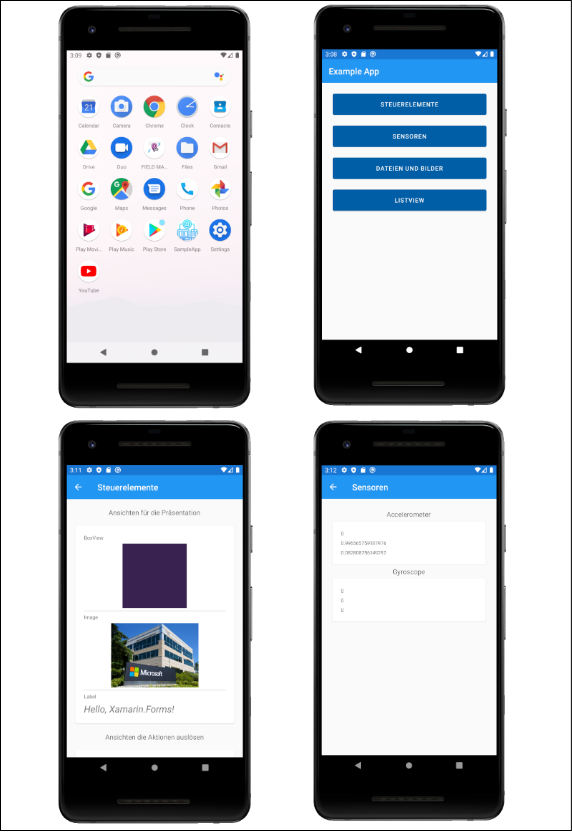
\includegraphics[width=\textwidth,keepaspectratio]{Images/Screenshot/AndroidScrenshotI.png}
 \caption[]{Test Objekt Screenshots I}
\end{figure}


\begin{figure}[!ht]
 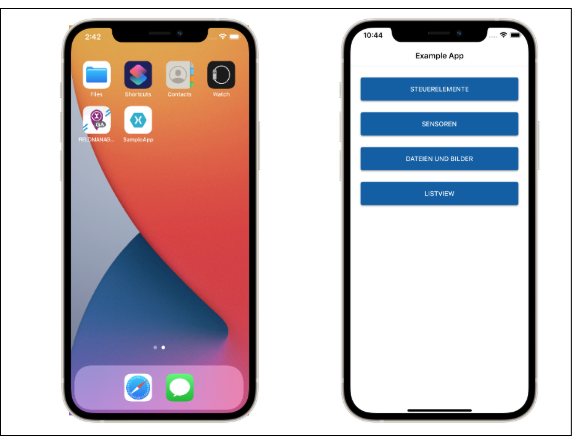
\includegraphics[width=\textwidth,keepaspectratio]{Images/Screenshot/AppIconAndMenu.png}
 \caption[]{Test Objekt Screenshots III}
\end{figure}

\begin{figure}[!ht]
 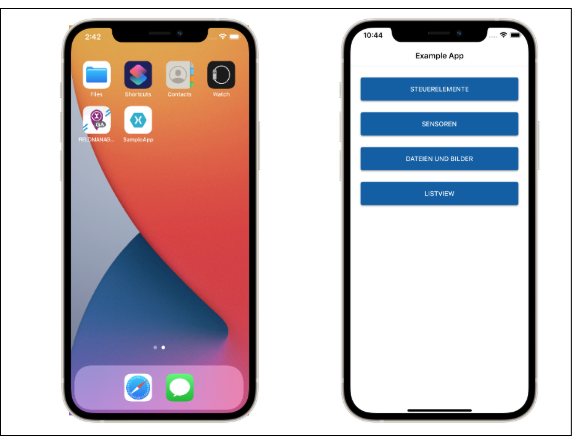
\includegraphics[width=\textwidth,keepaspectratio]{Images/Screenshot/AppIconAndMenu.png}
 \caption[]{Test Objekt Screenshots IV}
\end{figure}





  \printEidesstattlicheErklaerung % Setzt die eidesstattlichen Erklärung
\end{document}
